% Created 2021-04-01 qui 19:23
% Intended LaTeX compiler: pdflatex
\documentclass{SelfArx}
  \usepackage[T1]{fontenc}
\usepackage[utf8]{inputenc}
\usepackage{booktabs}
\renewcommand{\arraystretch}{1.1} % Unclear
\usepackage{graphicx}
\usepackage{float}
\usepackage{amsmath}
\usepackage{csquotes}
\setlength{\fboxrule}{0.75pt} % Width of the border around the abstract
\usepackage{longtable}
\definecolor{color1}{RGB}{0,0,90} % Color of the article title and sections
\definecolor{color2}{RGB}{0,20,20} % Color of the boxes behind the abstract and headings
\usepackage[portuguese, english]{babel} % Specify a different language here - english by default
\usepackage{lipsum} % Required to insert dummy text. To be removed otherwise
\usepackage[backend=biber,%
style = abnt,%
noslsn, %
isbn = false,
url = false,
extrayear, %
uniquename=init,%
giveninits, %
justify, %
sccite,%
scbib, %
sorting=nyt,
% mergedate=compact,
% natbib=true,
repeattitles, %
maxcitenames=3]{biblatex}
\AtEveryBibitem{%
\clearfield{urlyear}
\clearfield{urlmonth}
\clearfield{note}
\clearfield{issn} % Remove issn
\clearfield{doi} % Remove doi
\ifentrytype{online}{}{% Remove url except for @online
\clearfield{url}
}
}
\usepackage{multirow, numprint}
\date{}
\title{Dados: O PIB da pandemia e cenários para 2021}
\begin{document}

\JournalInfo{Nota de Conjuntura No 16} % Journal information
\Archive{} % Additional notes (e.g. copyright, DOI, review/research article)

\Authors{Pedro Paulo Zahluth Bastos\textsuperscript{1}*, Lorena Dourado\textsuperscript{2}, Gabriel Petrini\textsuperscript{3}, Antônio Ibarra\textsuperscript{3}}} % Authors
\affiliation{\textsuperscript{1}\textit{Professor do Instituto de Economia Unicamp}} % Author affiliation
\affiliation{\textsuperscript{2}\textit{Graduanda do Instituto de Economia Unicamp}} % Author affiliation
\affiliation{\textsuperscript{3}\textit{Doutorando do Instituto de Economia  Unicamp}} % Author affiliation
\affiliation{*\textbf{E-mail}: ppzbastos@gmail.com} % Corresponding author

\Keywords{Keyword1 --- Keyword2 --- Keyword3} % Keywords - if you don't want any simply remove all the text between the curly brackets
\newcommand{\keywordname}{Palavras-chave} % Defines the keywords heading name

\Abstract{
\begin{itemize}

\item Em março, havia risco de sucessão longa de quedas trimestrais do PIB, com círculo vicioso de contração de demanda, contração do crédito, falências de empresas e ampliação do desemprego e da pobreza.
\item O risco foi contornado com política anticíclica para sustentar renda, vínculos empregatícios e, tardiamente, ampliação do crédito (apesar do repasse da depreciação cambial).
\item A continuidade da pandemia limitou a retomada da demanda e do emprego em serviços em razão do risco de contágio, reafirmando a centralidade do controle da pandemia para a recuperação da economia (não há trade-off duradouro).
\item A magnitude da política anticíclica gera um risco enorme de um segundo mergulho em razão da retomada da lei do teto do gasto e da retirada brusca dos programas emergenciais.
\item Sem política anticíclica, aumento do desemprego e da pobreza serão dramáticos ainda que as exportações se recuperem em 2021.
\end{itemize}
}
\renewcommand{\abstractname}{Sumário Executivo} % Defines the keywords heading name
\flushbottom % Makes all text pages the same height
\maketitle % Print the title and abstract box
\thispagestyle{empty} % Removes page numbering from the first page
\onecolumn
\bibliography{refs}

\section*{Indicadores de antecedente}
\label{sec:org581c634}
\subsection*{IBC-Br (acumulado 12 meses vs 12 meses anteriores)}
\label{sec:org4f4e14d}

\begin{center}
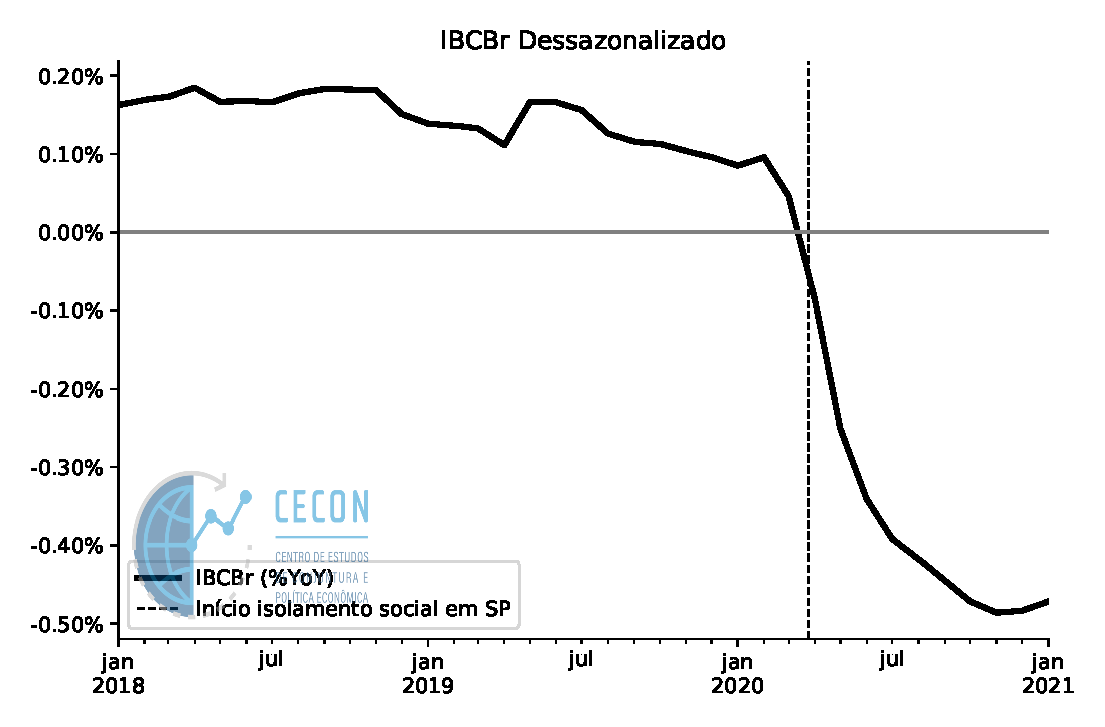
\includegraphics[width=.9\linewidth]{./figs/Antecedente/IBCBr.pdf}
\end{center}

\subsection*{Tráfego de veículos pesados nas estradas pedagiadas - ABCR - Dados dessazonalizados}
\label{sec:orgd3e4e1e}


\begin{center}
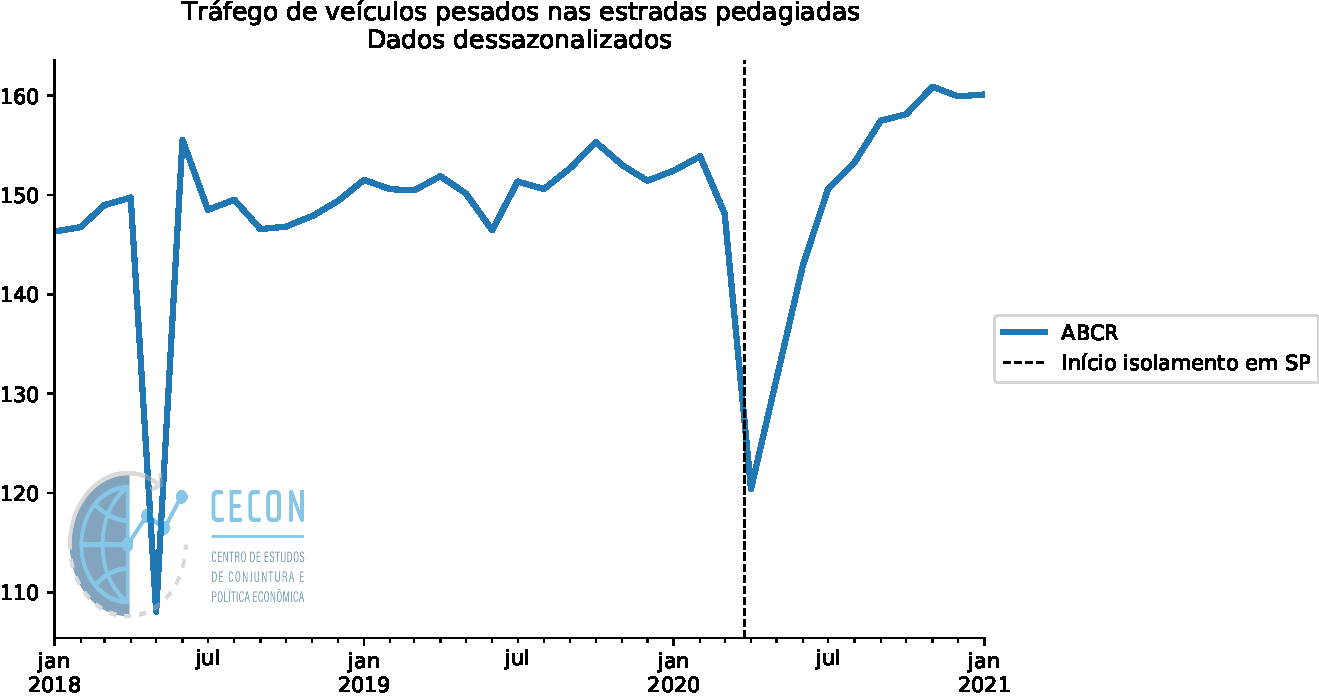
\includegraphics[width=.9\linewidth]{./figs/Setoriais/TrafegoPedagio.pdf}
\end{center}


\section*{Dados de alta frequência}
\label{sec:org3865738}

\subsection*{Bloomberg adaptado ao COVID-19 (\href{https://www.bloomberg.com/news/articles/2020-11-13/alternative-data-show-activity-crashes-as-virus-resurges-chart}{Link})}
\label{sec:orga1af766}

\subsection*{Google Reports: Brasil}
\label{sec:org69354b3}

\begin{center}
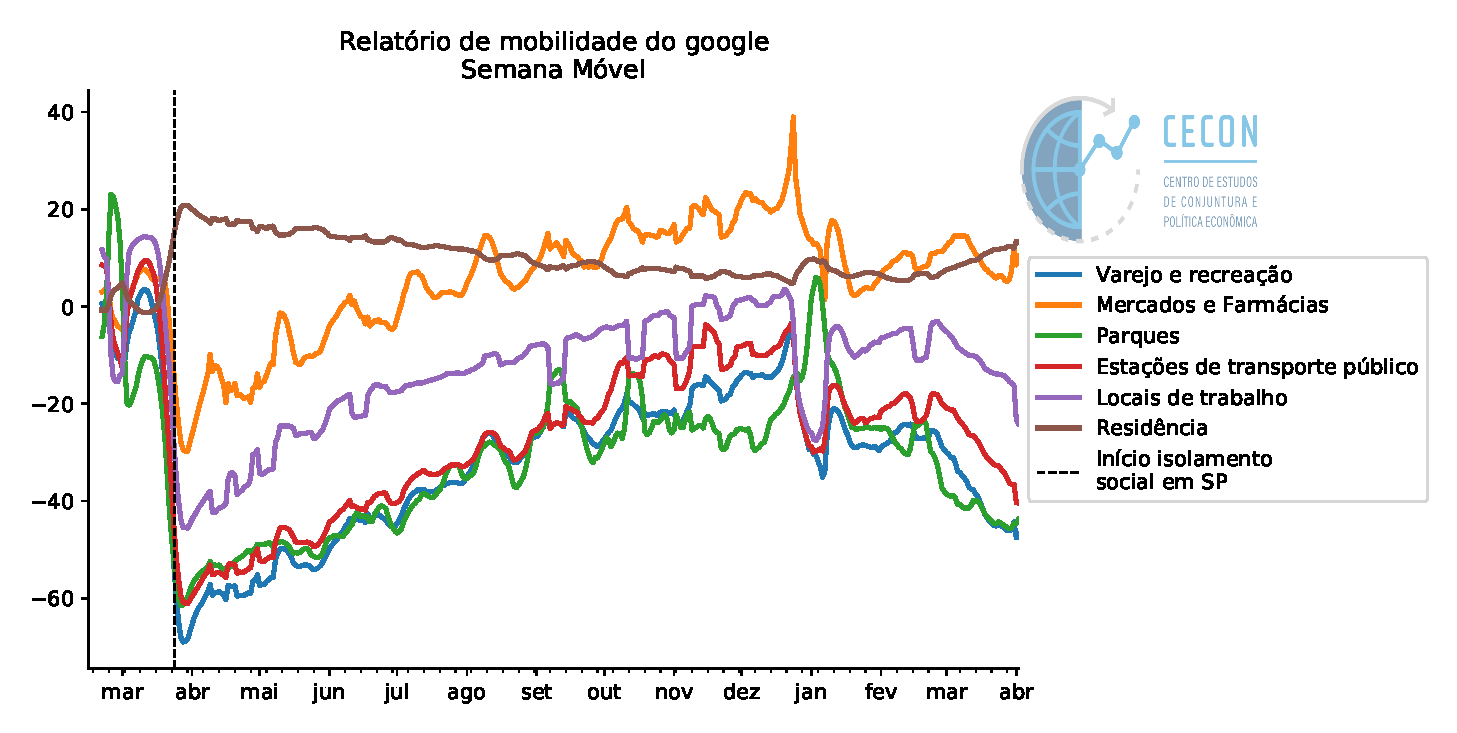
\includegraphics[width=.9\linewidth]{./figs/Granulares/GoogleReport_Brasil.pdf}
\end{center}

\subsection*{Apple: Tendências de mobilidade}
\label{sec:org83fd206}

\begin{center}
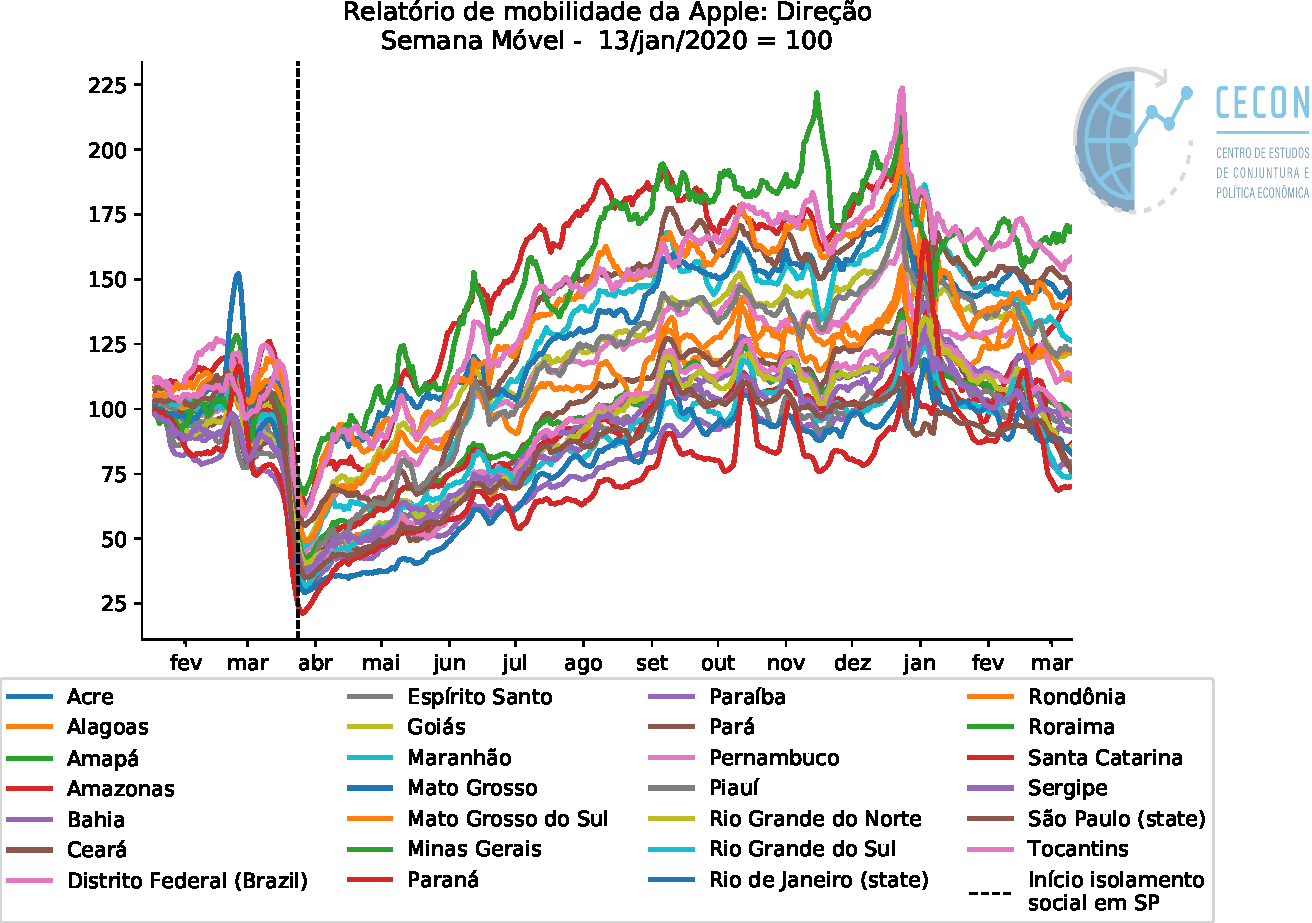
\includegraphics[width=.9\linewidth]{./figs/Granulares/AppleReport_Brasil.pdf}
\end{center}

\subsection*{Waze: \(\Delta \%\) Km}
\label{sec:orgcfe4818}

\begin{center}
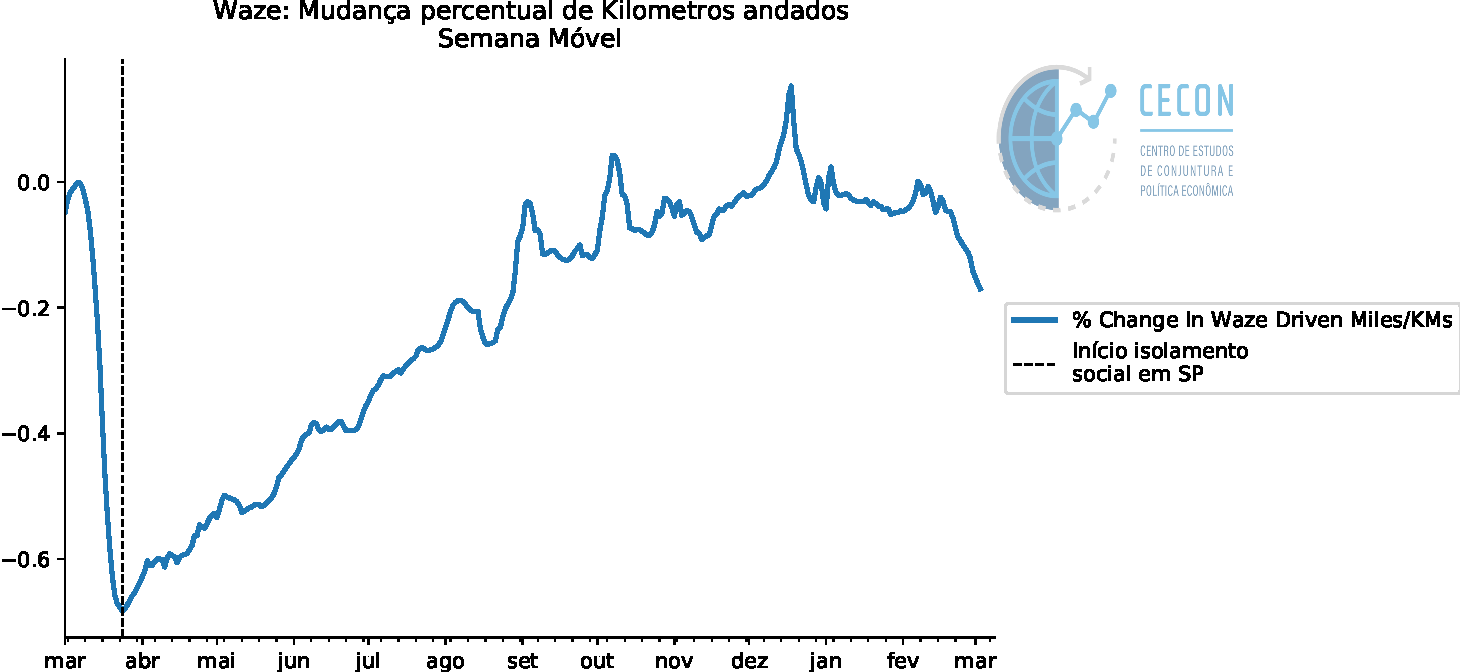
\includegraphics[width=.9\linewidth]{./figs/Granulares/Waze_Brasil.pdf}
\end{center}

\subsection*{TomTom: Congestionamento}
\label{sec:org9dcba9c}

\begin{center}
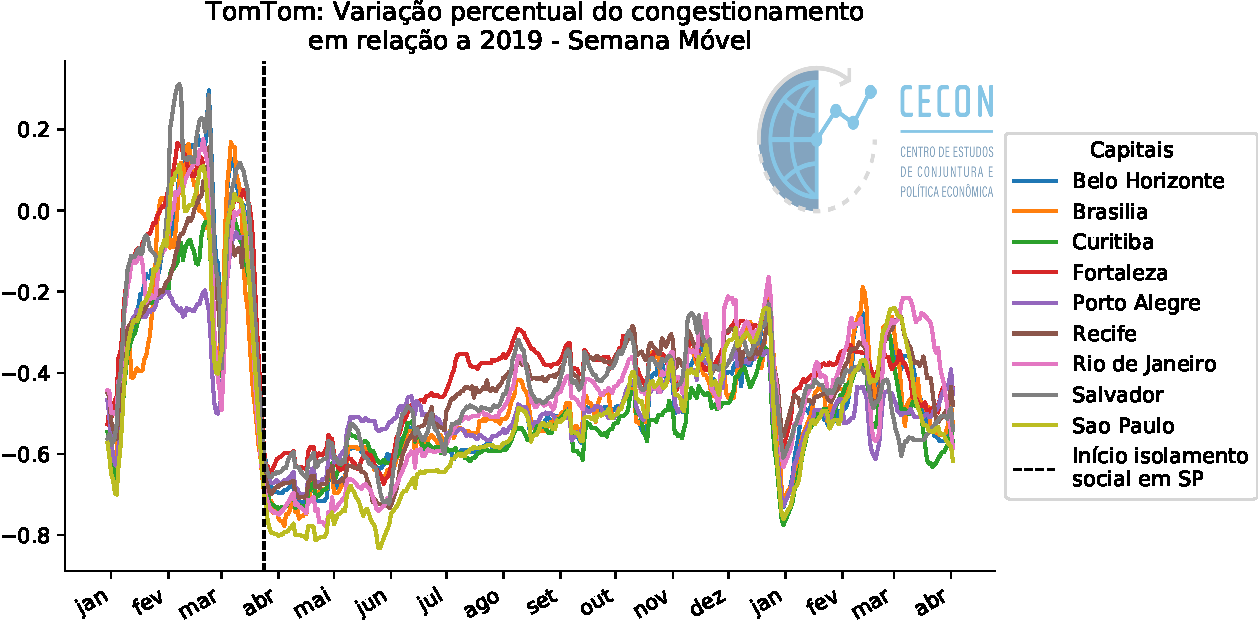
\includegraphics[width=.9\linewidth]{./figs/Granulares/TomTom_Brasil.pdf}
\end{center}

\section*{Atividade}
\label{sec:org6c3bfb2}



\subsection*{Trimestre Contra trimestre imediatamente anterior}
\label{sec:org772cad8}

\begin{center}
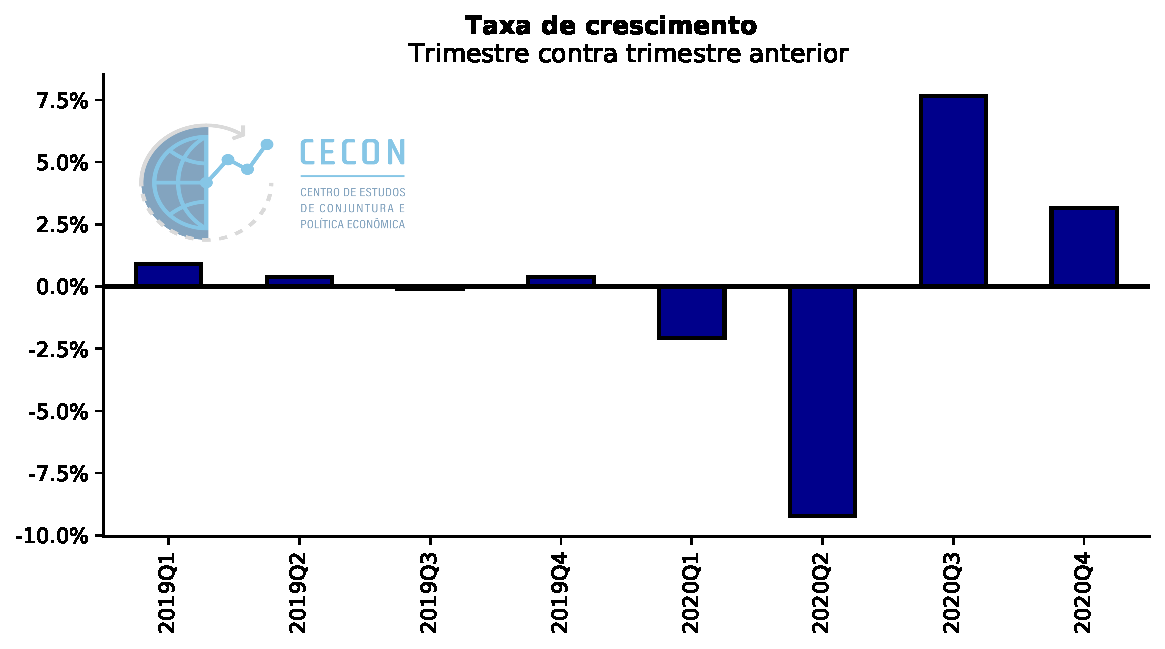
\includegraphics[width=.9\linewidth]{./figs/PIB/PIB.pdf}
\end{center}

\subsection*{Trimestre Contra mesmo trimestre do ano anterior}
\label{sec:org259c4ce}

\begin{center}
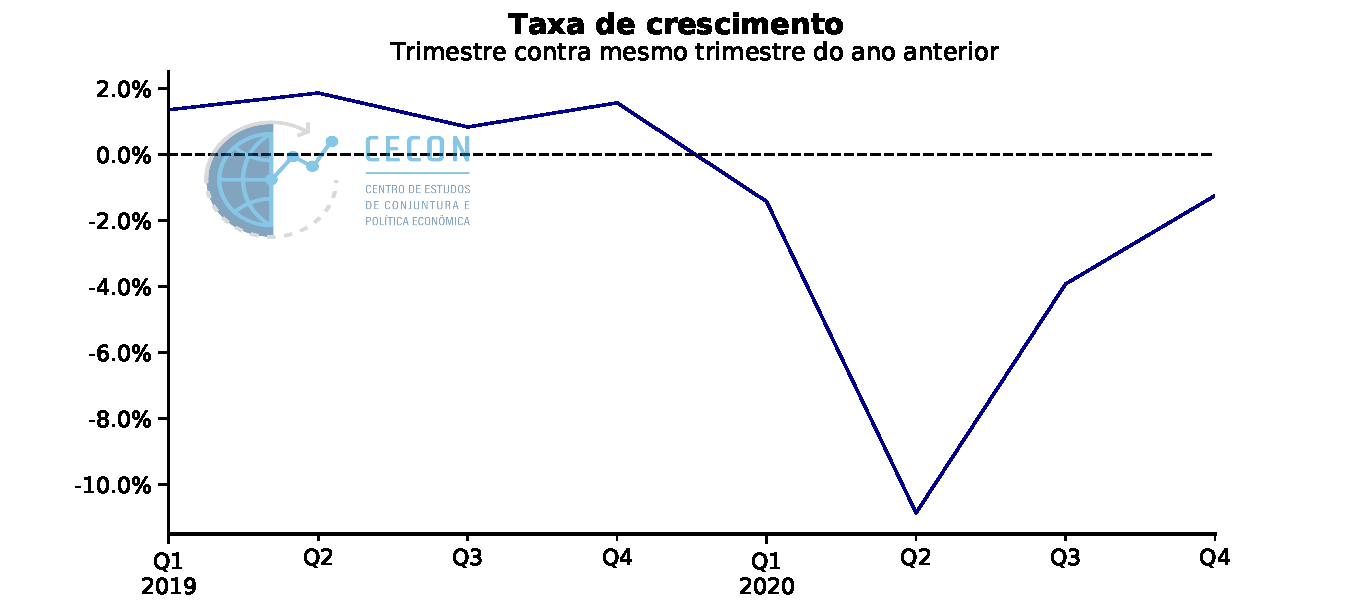
\includegraphics[width=.9\linewidth]{./figs/PIB/PIB_YoY.pdf}
\end{center}

\subsection*{Agropecuária}
\label{sec:org5455a42}

\begin{center}
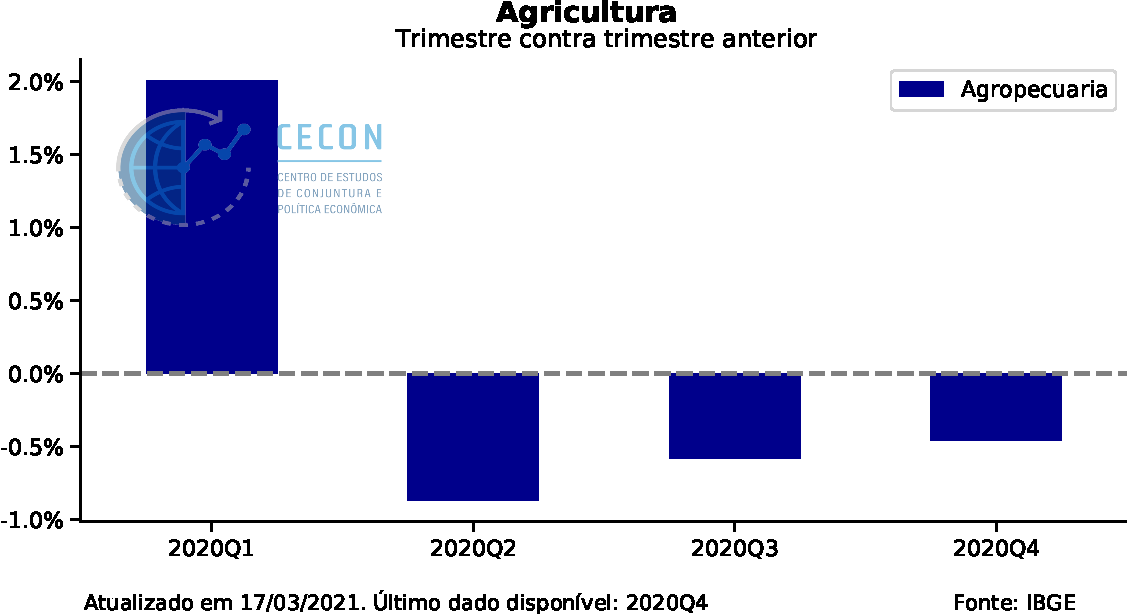
\includegraphics[width=.9\linewidth]{./figs/PIB/Agropecuaria.pdf}
\end{center}

\subsection*{Indústria}
\label{sec:org8a78c99}

\begin{center}
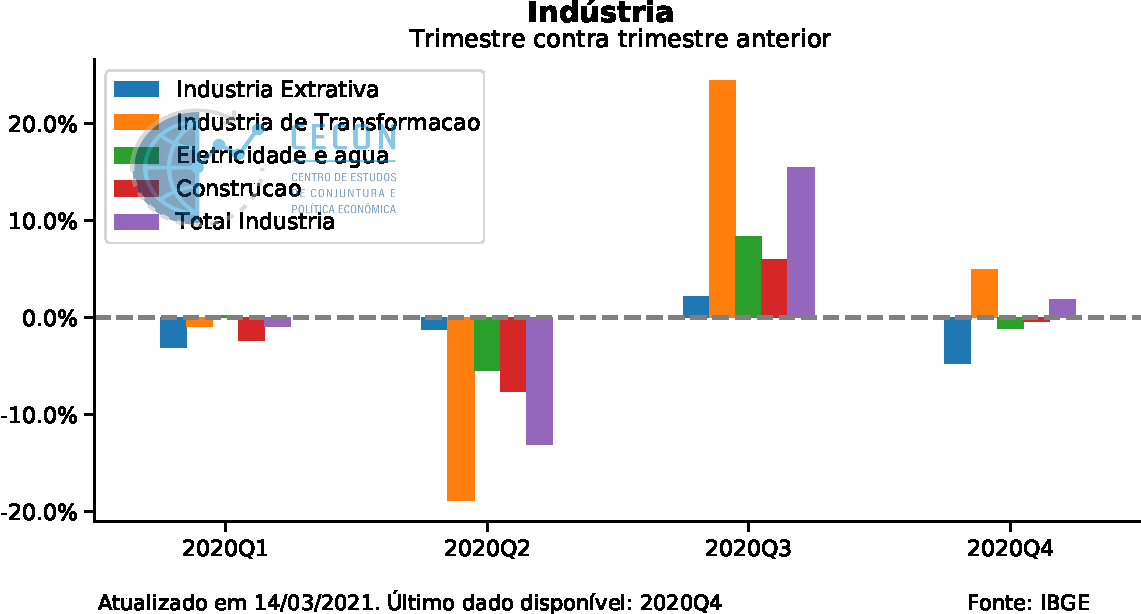
\includegraphics[width=.9\linewidth]{./figs/PIB/Industria.pdf}
\end{center}


\subsection*{Serviços}
\label{sec:org0a25602}

\begin{center}
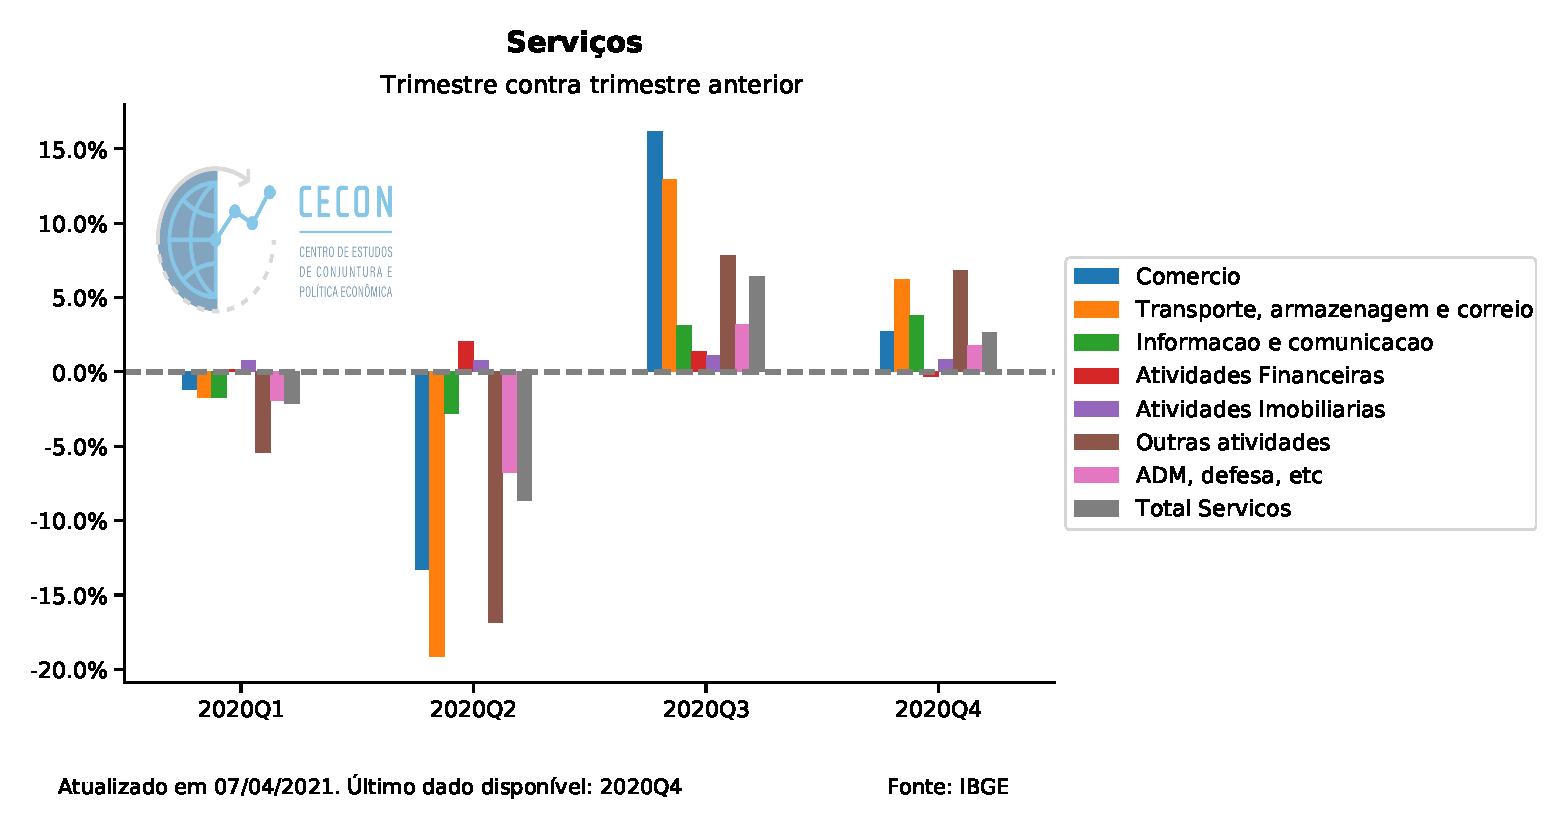
\includegraphics[width=.9\linewidth]{./figs/PIB/Servicos.pdf}
\end{center}

\subsection*{Demanda}
\label{sec:orge84025f}

\begin{center}
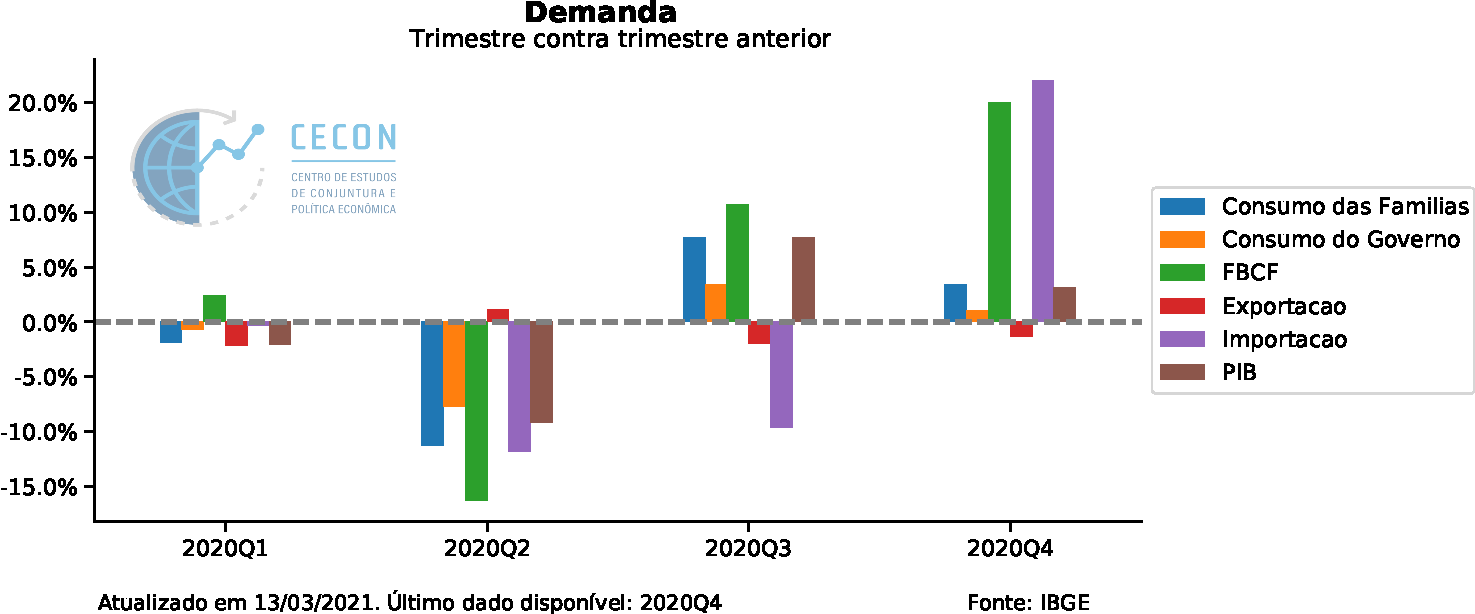
\includegraphics[width=.9\linewidth]{./figs/PIB/Demanda.pdf}
\end{center}

\subsection*{Oferta}
\label{sec:org8f5f178}


\begin{center}
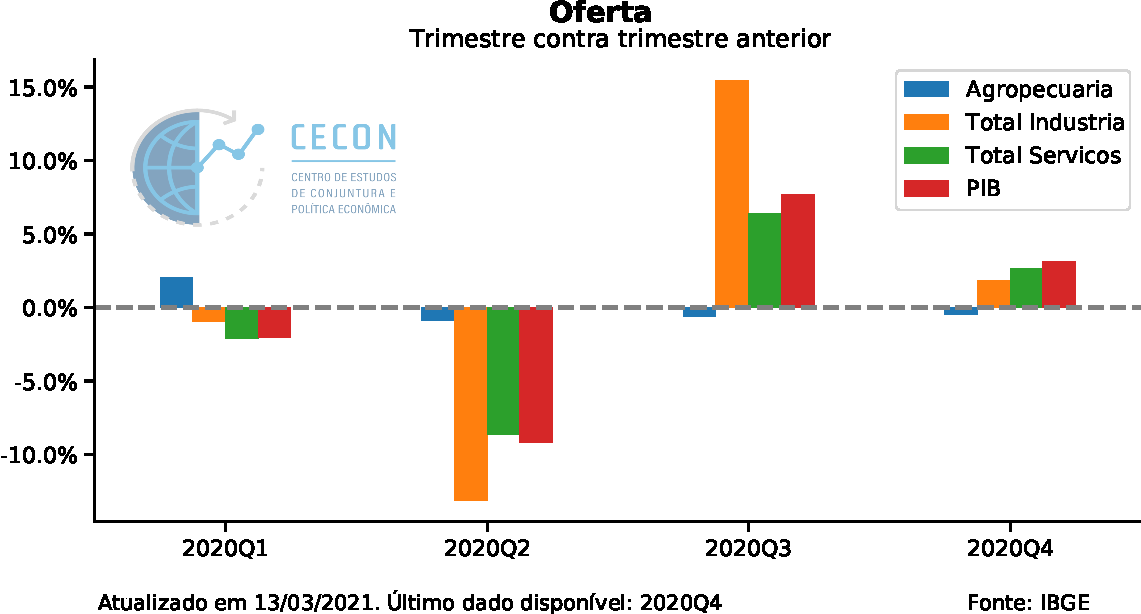
\includegraphics[width=.9\linewidth]{./figs/PIB/Oferta.pdf}
\end{center}


\subsection*{Contribuição para variação: Demanda}
\label{sec:orgbc35319}

\begin{center}
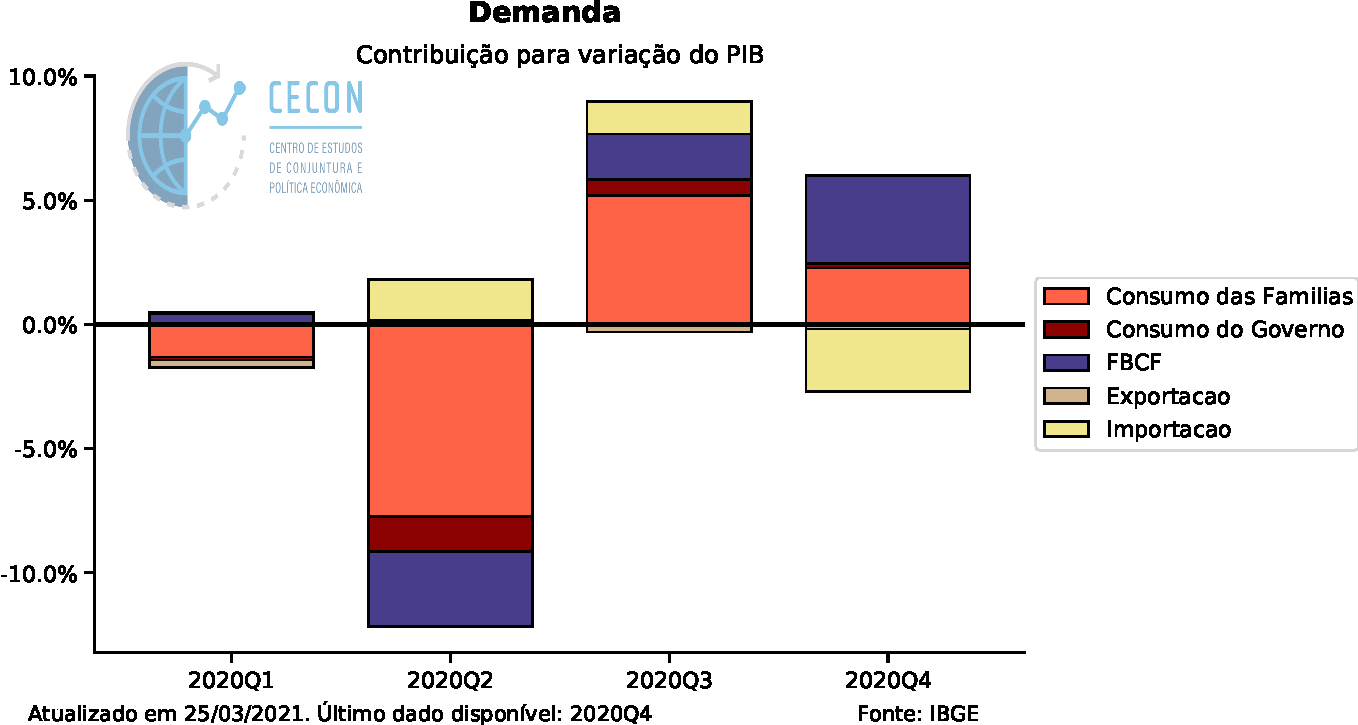
\includegraphics[width=.9\linewidth]{./figs/PIB/Contrib_Demanda.pdf}
\end{center}

\subsection*{Contribuição para variação: Oferta}
\label{sec:orgd9181b4}

\begin{center}
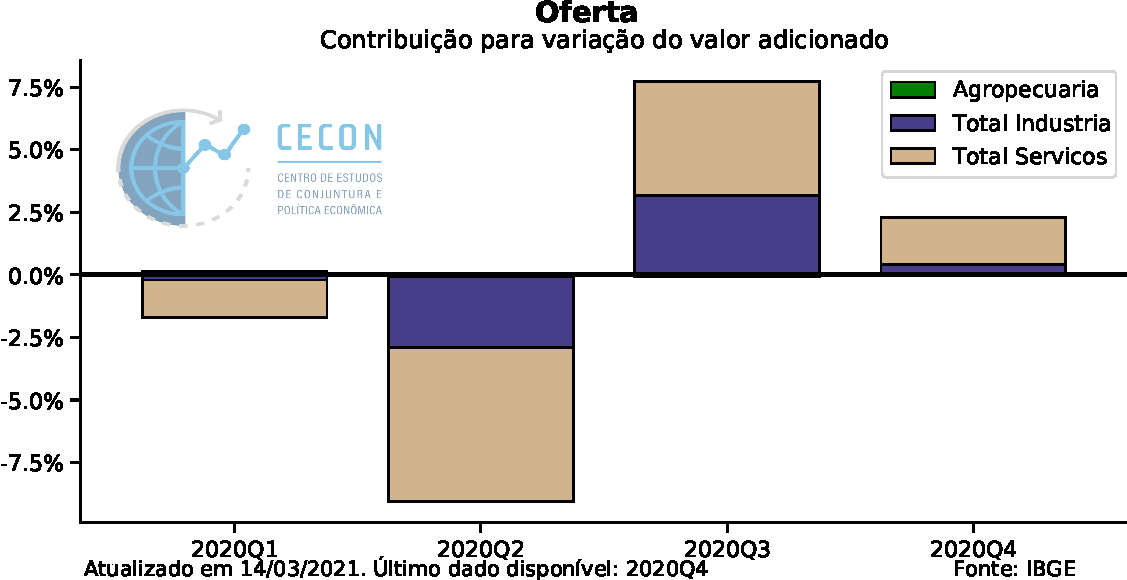
\includegraphics[width=.9\linewidth]{./figs/PIB/Contrib_Oferta.pdf}
\end{center}


\subsection*{Contribuição para variação: Serviços}
\label{sec:org52422fe}

\begin{center}
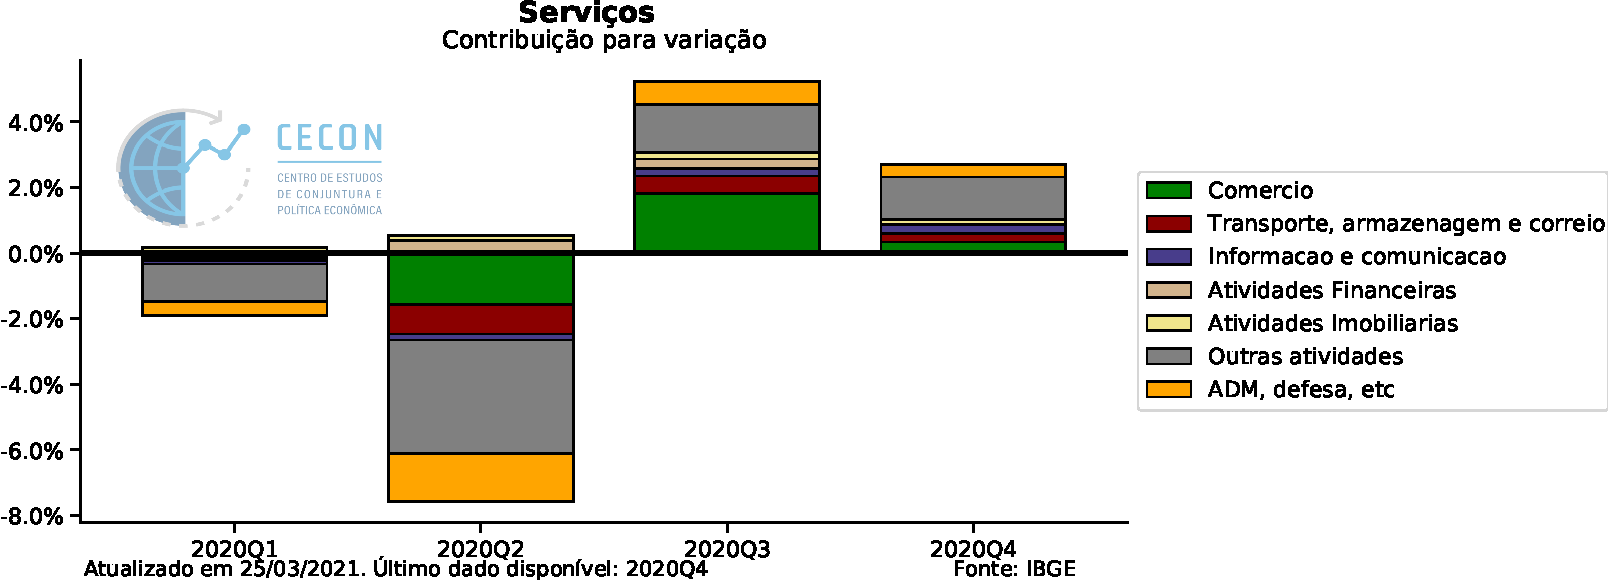
\includegraphics[width=.9\linewidth]{./figs/PIB/Contrib_Servicos.pdf}
\end{center}

\subsection*{Acumulado no ano (sem ajuste)}
\label{sec:orgecb8db2}

\subsubsection*{Serviços}
\label{sec:org7aad43e}

\begin{center}
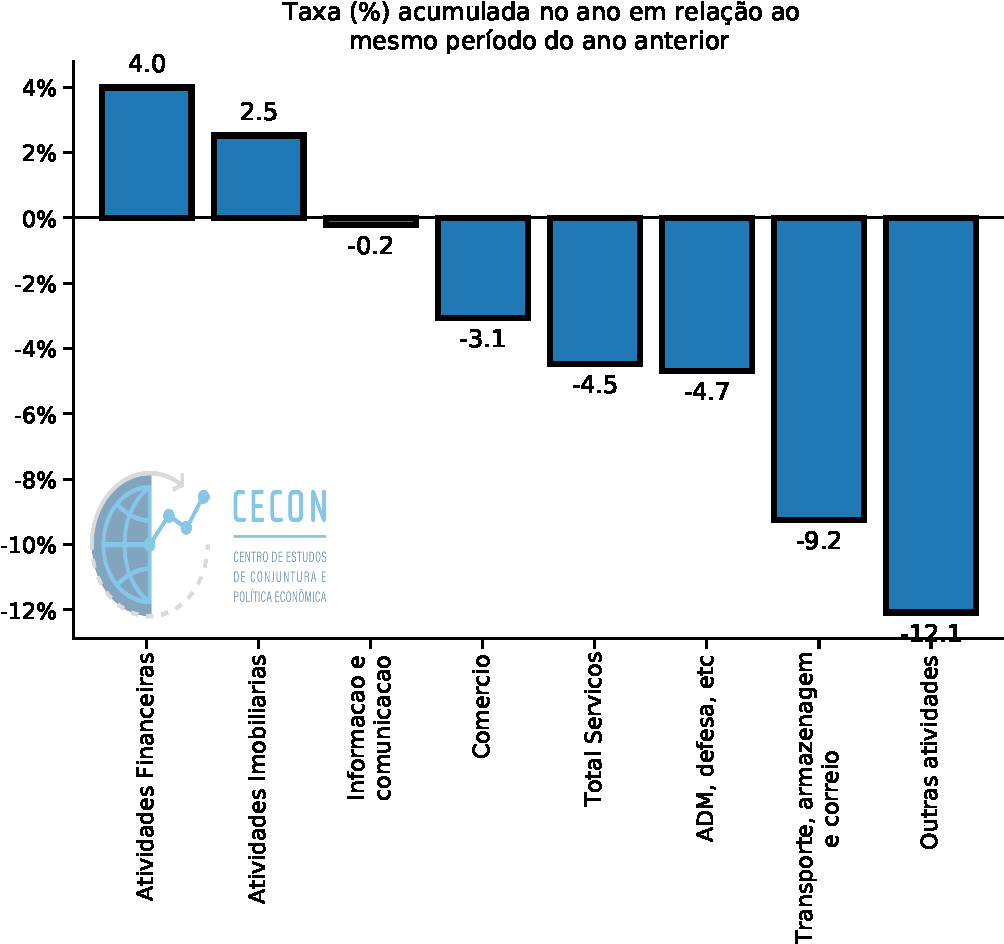
\includegraphics[width=.9\linewidth]{./figs/PIB/Servicos_Acum.pdf}
\end{center}

\subsubsection*{Serviços (comparação com ano anterior)}
\label{sec:org70f9d1b}

\begin{center}
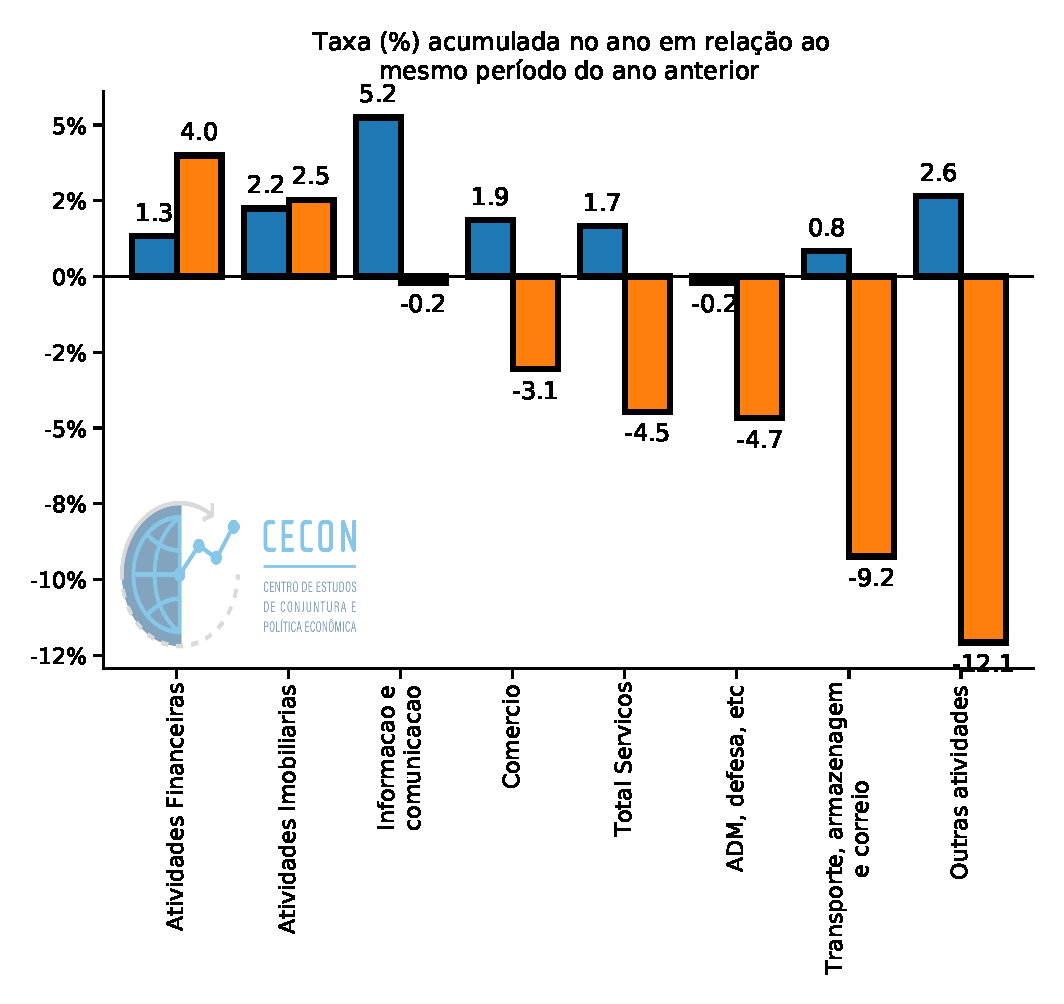
\includegraphics[width=.9\linewidth]{./figs/PIB/Servicos_Acum_Comparativo.pdf}
\end{center}

\subsubsection*{Demanda}
\label{sec:orgc39f3e2}

\begin{center}
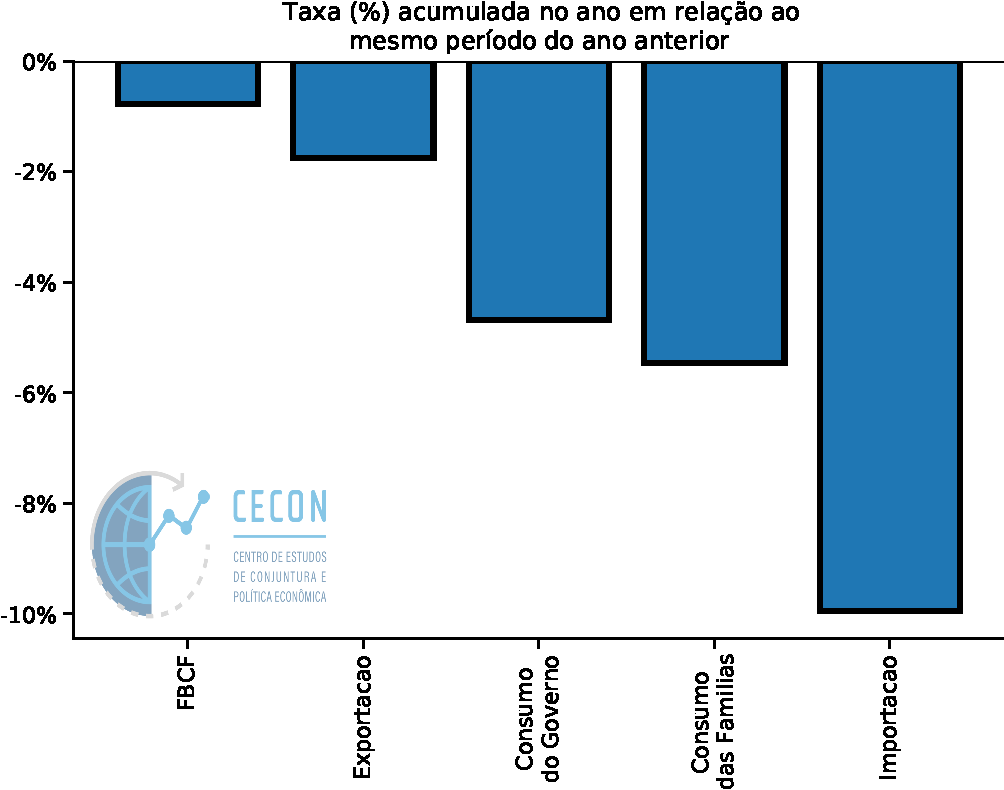
\includegraphics[width=.9\linewidth]{./figs/PIB/Demanda_Acum.pdf}
\end{center}

\subsubsection*{Demanda (comparação com ano anterior)}
\label{sec:orgcac6311}

\begin{center}
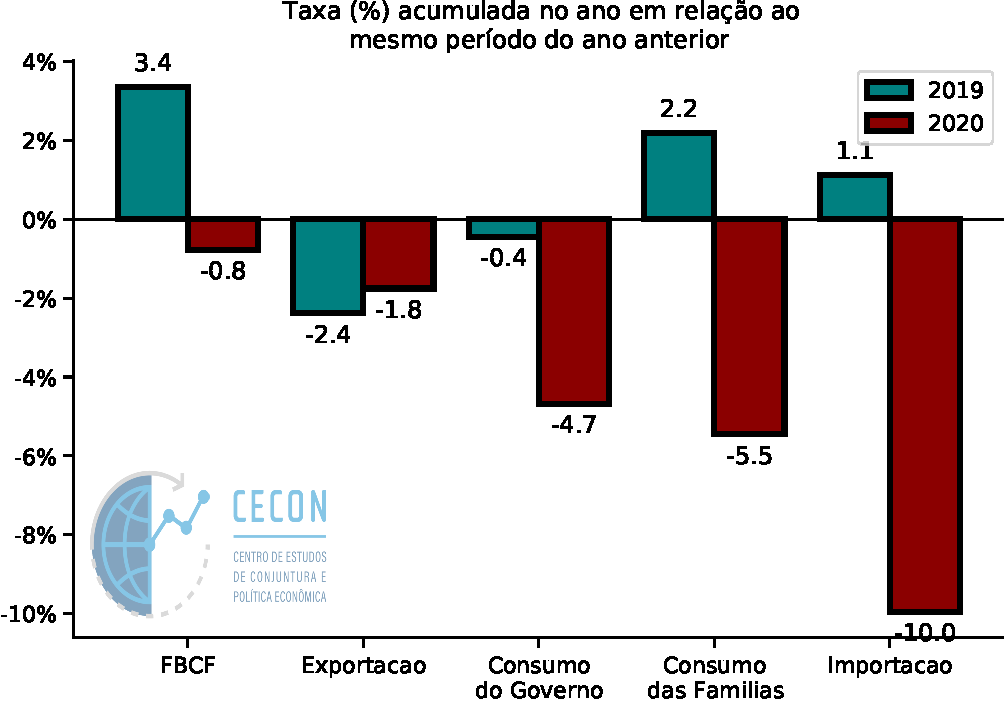
\includegraphics[width=.9\linewidth]{./figs/PIB/Demanda_Acum_Comparativo.pdf}
\end{center}

\subsubsection*{PIB}
\label{sec:orgdd73238}

\begin{center}
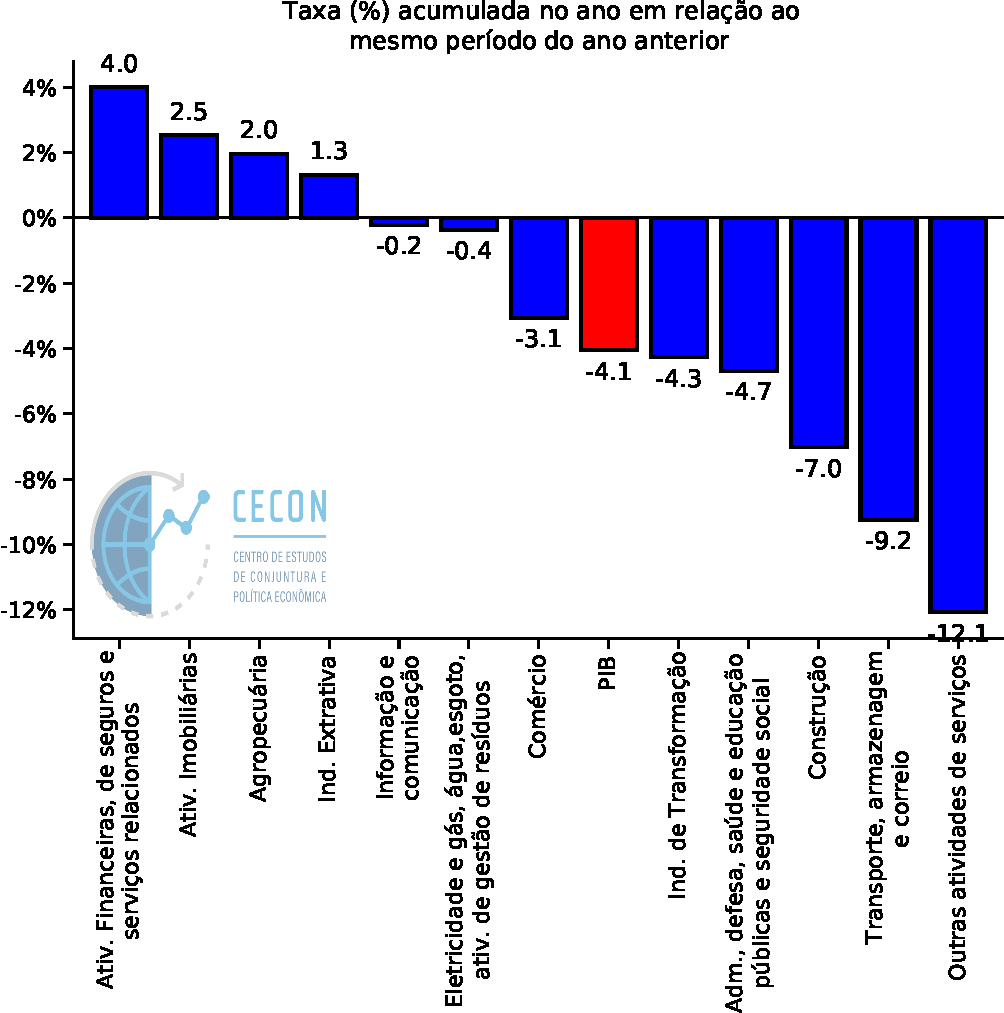
\includegraphics[width=.9\linewidth]{./figs/PIB/PIB_Acum.pdf}
\end{center}

\section*{Crédito}
\label{sec:org52e7f4b}

\subsection*{Endividamento das famílias}
\label{sec:orgfb7f6f6}

\begin{center}
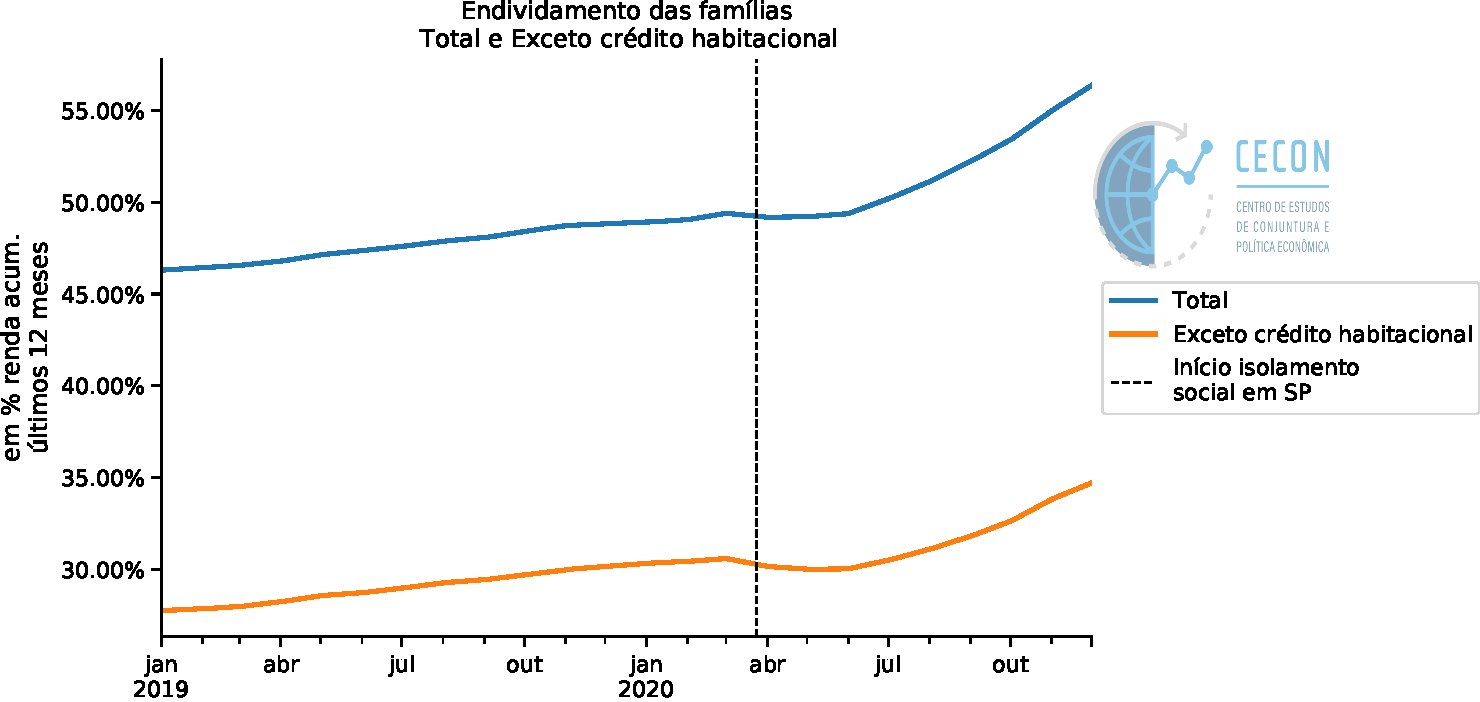
\includegraphics[width=.9\linewidth]{./figs/Credito/EndividamentoFamilias.pdf}
\end{center}


\subsection*{Saldo Pessoal Jurídica - Nível}
\label{sec:org318c149}

\begin{center}
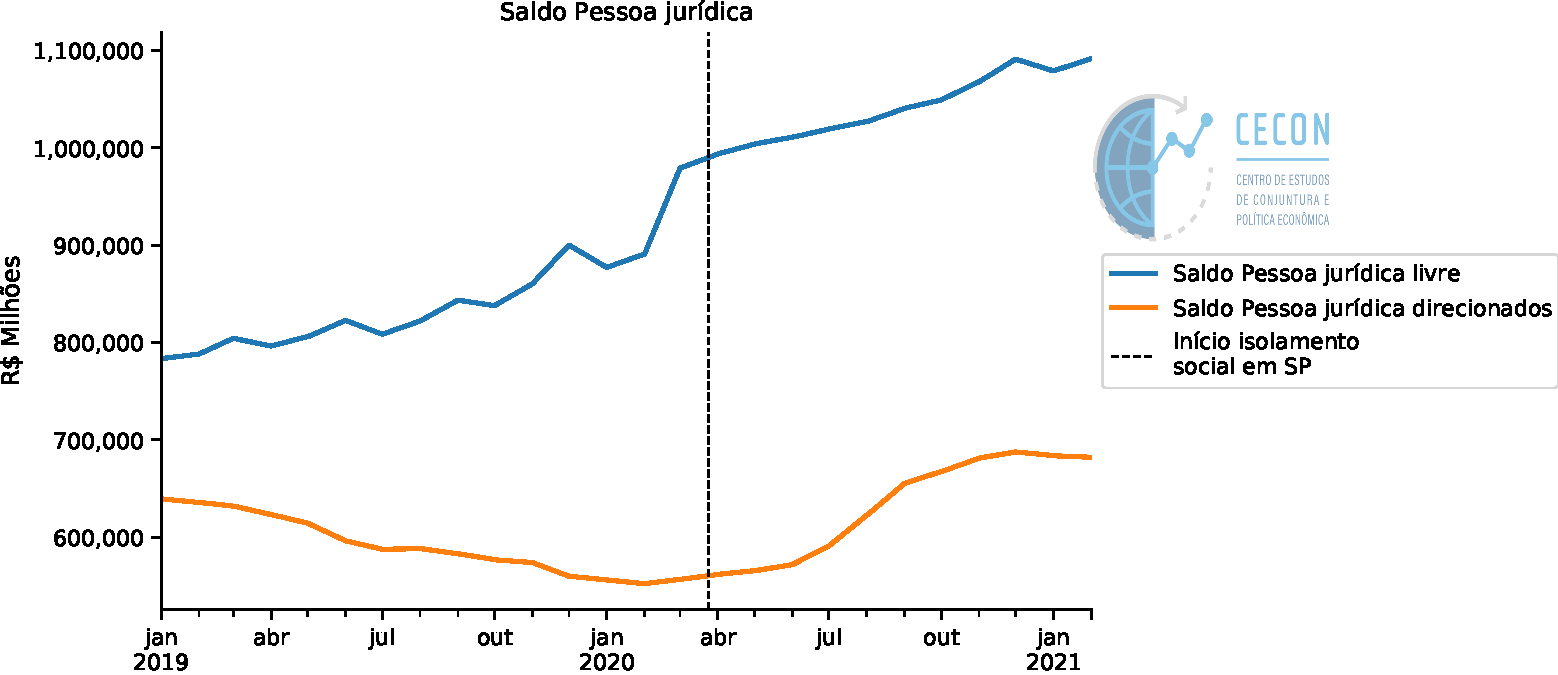
\includegraphics[width=.9\linewidth]{./figs/Credito/SaldoPJ.pdf}
\end{center}



\subsection*{Saldo Pessoa Jurídica - em \% do PIB}
\label{sec:orga711f1b}
\begin{center}
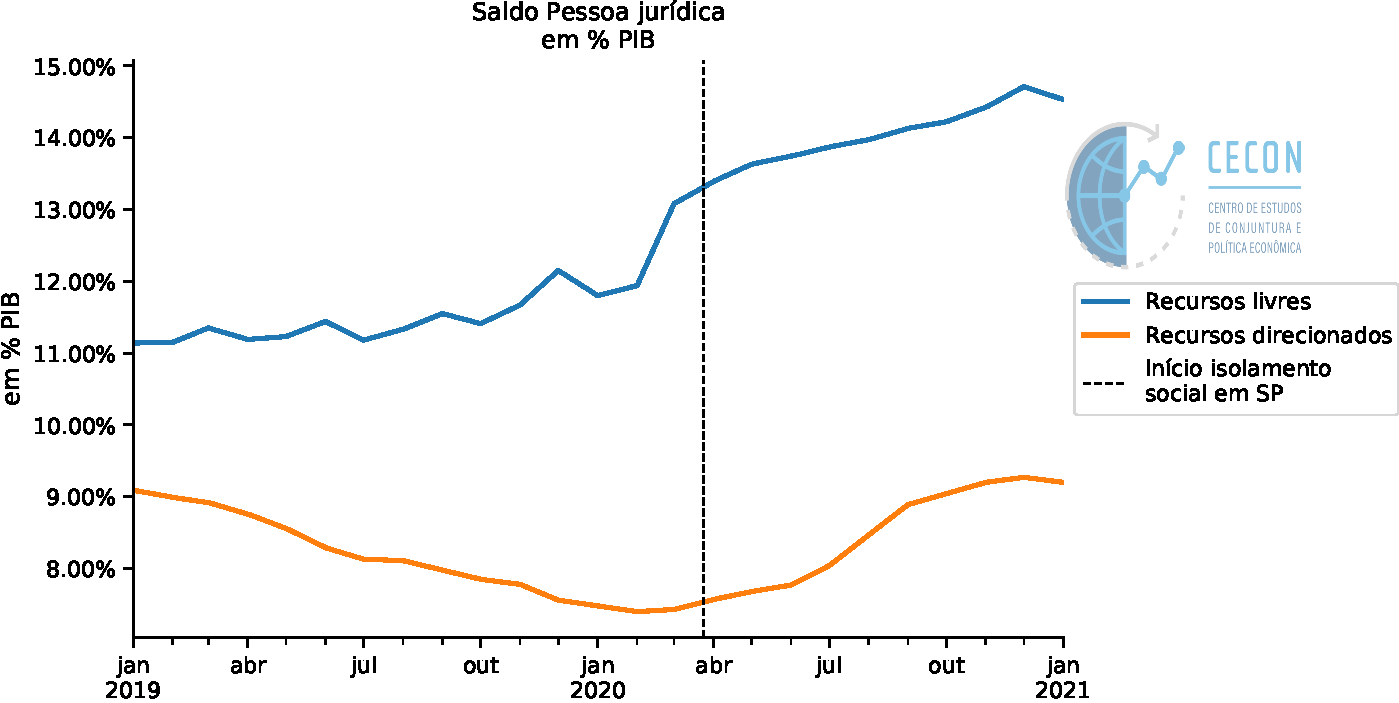
\includegraphics[width=.9\linewidth]{./figs/Credito/SaldoPJ_PIB.pdf}
\end{center}

\subsection*{Saldo Pessoa física - Nível}
\label{sec:orgd4e1103}

\begin{center}
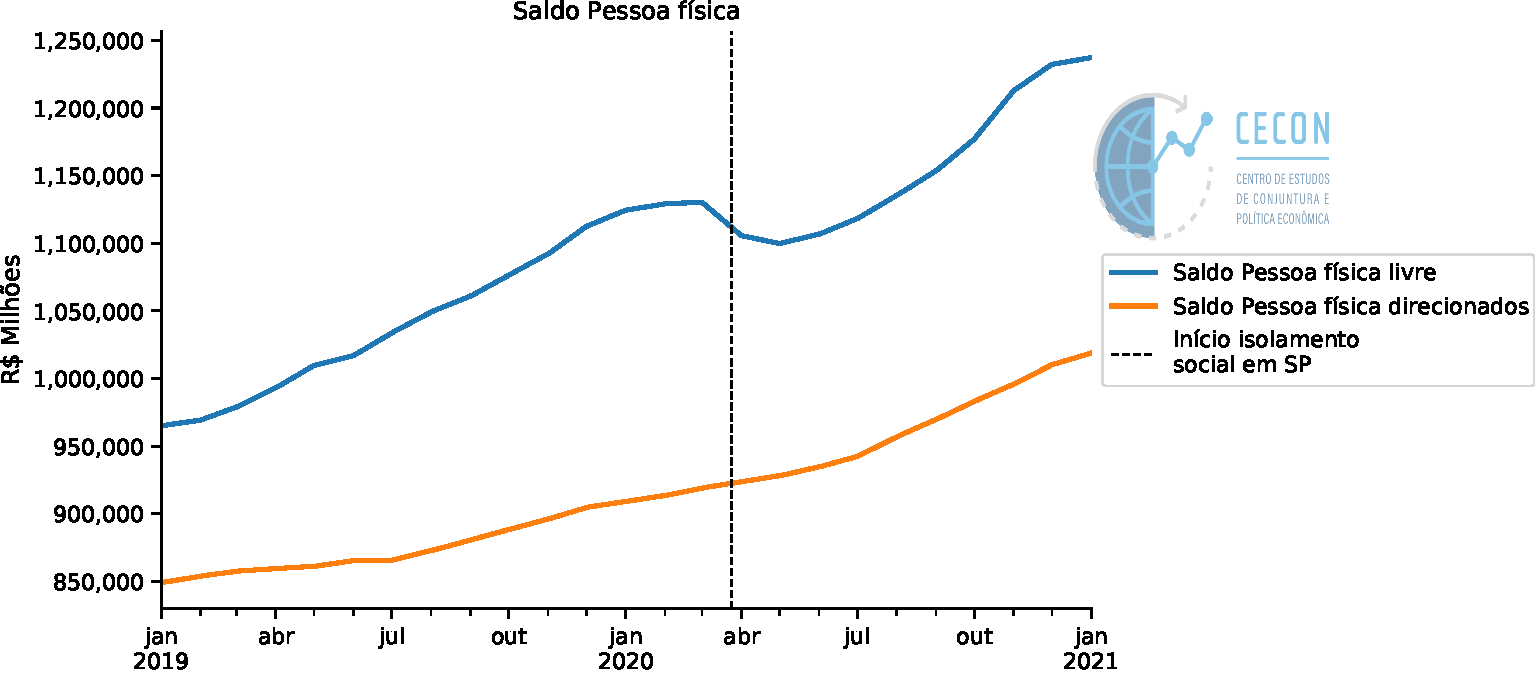
\includegraphics[width=.9\linewidth]{./figs/Credito/SaldoPF.pdf}
\end{center}


\subsection*{Saldo Pessoa física - em \% do PIB}
\label{sec:org4a0a622}

\begin{center}
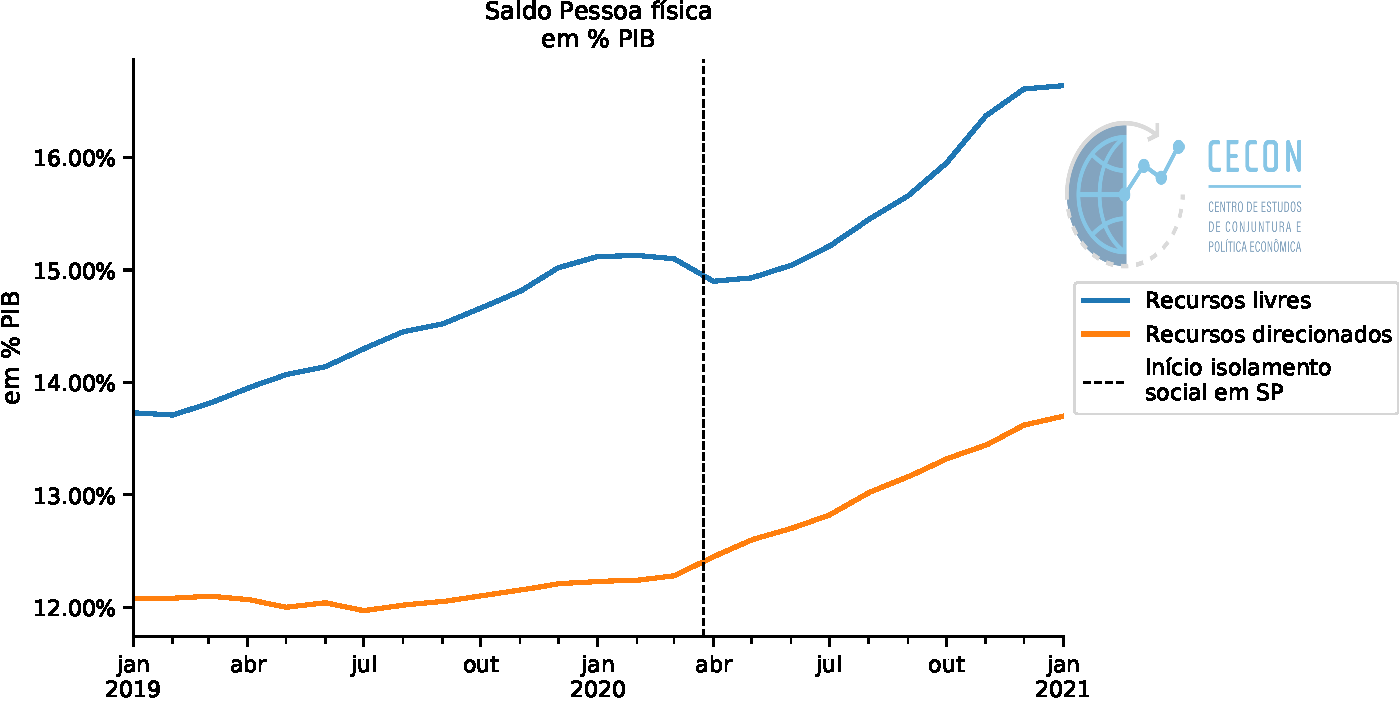
\includegraphics[width=.9\linewidth]{./figs/Credito/SaldoPF_PIB.pdf}
\end{center}


\subsection*{Crédito ampliado em \% do Total}
\label{sec:org27523b4}

\begin{center}
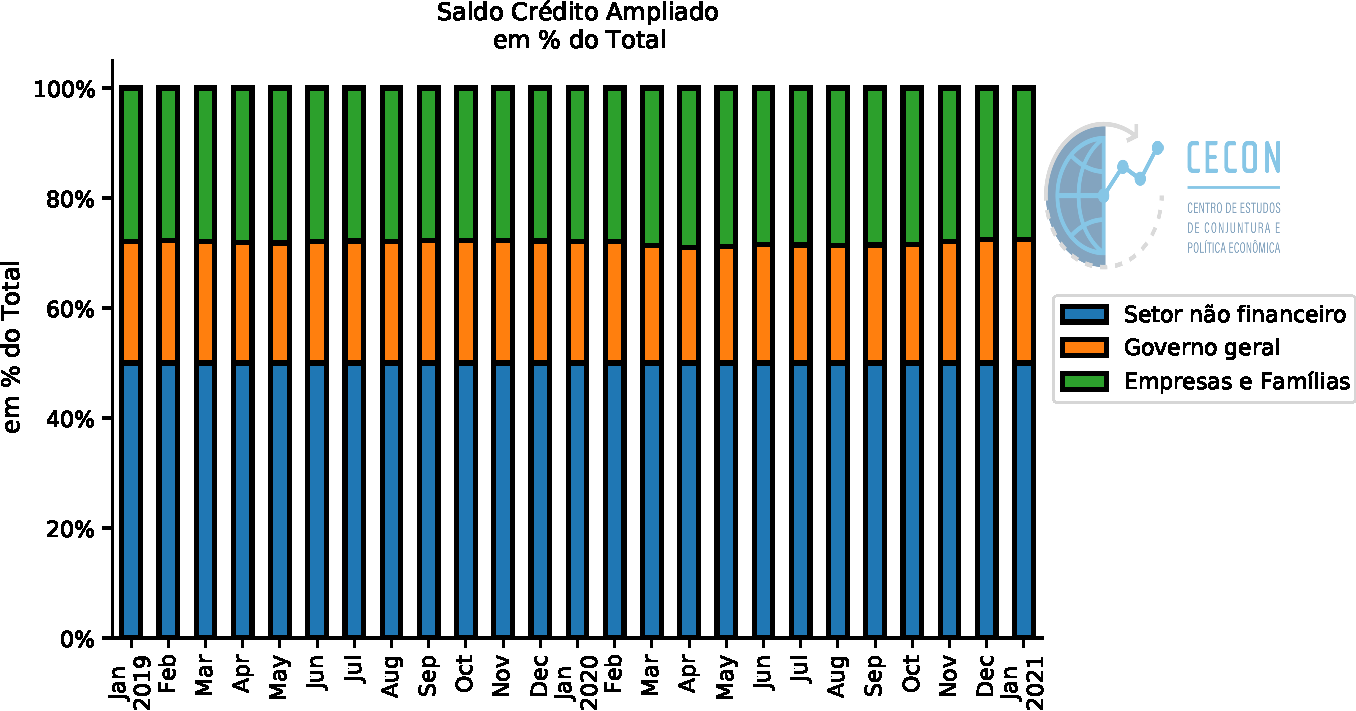
\includegraphics[width=.9\linewidth]{./figs/Credito/SaldoCreditoAmpliado_Total.pdf}
\end{center}

\subsection*{Indicadores de aprovação de crédito}
\label{sec:orga3e2a8f}

\begin{center}
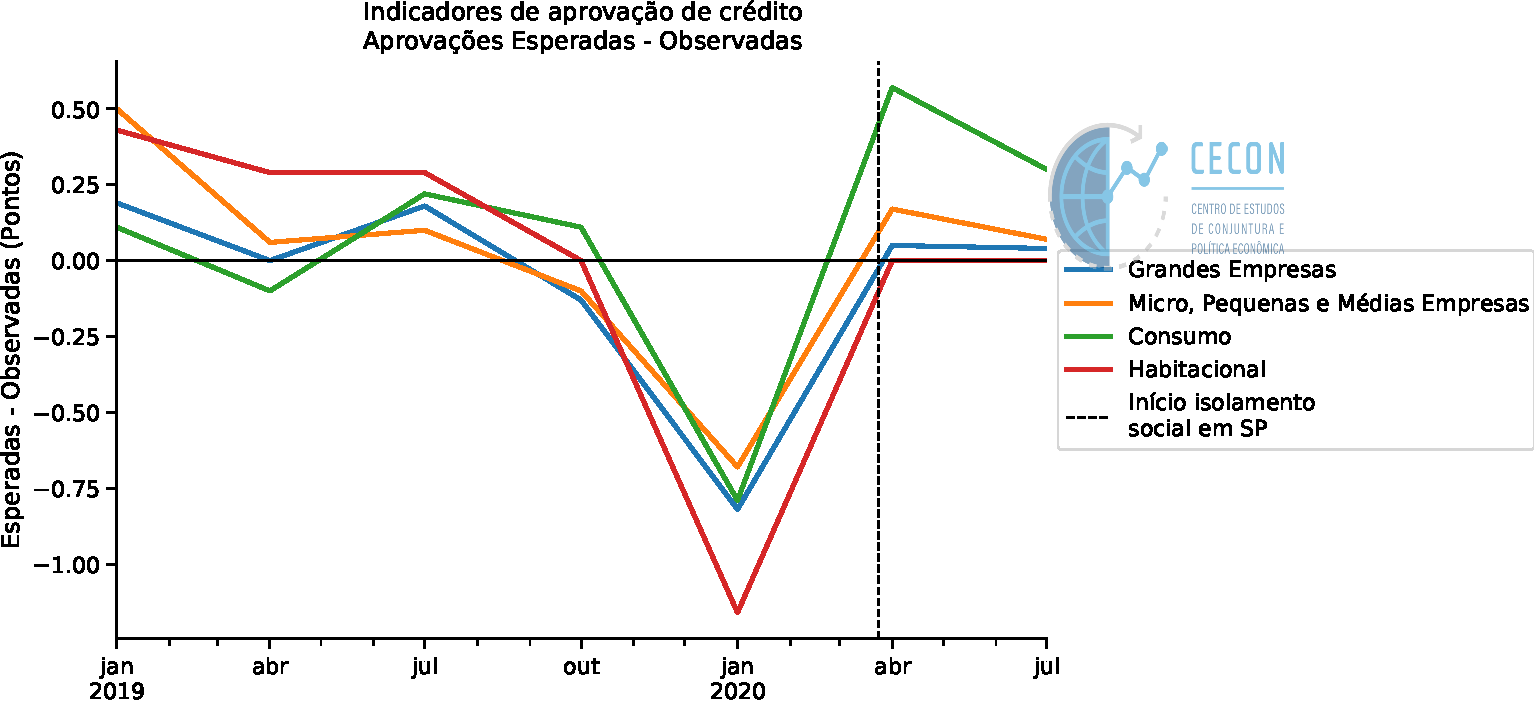
\includegraphics[width=.9\linewidth]{./figs/Credito/PTC.pdf}
\end{center}

\subsection*{Recolhimentos compulsórios de instituições financeiras}
\label{sec:org5eb86e0}

\begin{center}
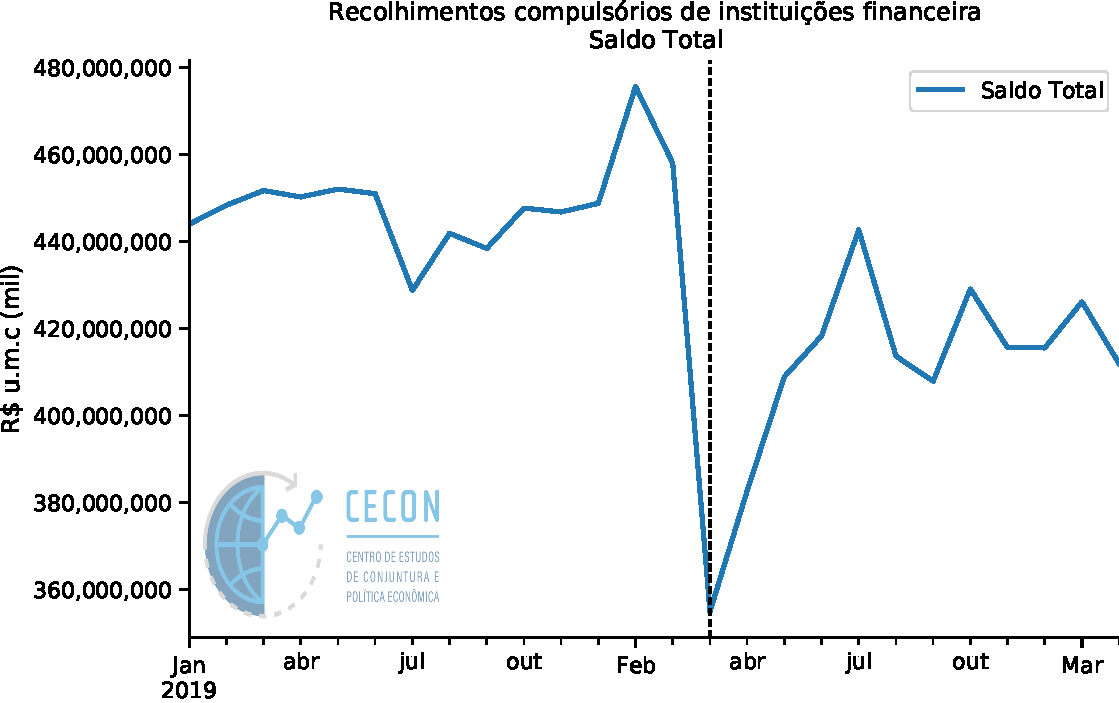
\includegraphics[width=.9\linewidth]{./figs/Credito/Recolhimentos_Total.pdf}
\end{center}

\section*{Índices de atividade setoriais}
\label{sec:orgdfe92d5}


\subsection*{Pesquisa Mensal do Comércio (PMC)}
\label{sec:org648bbc1}

\begin{center}
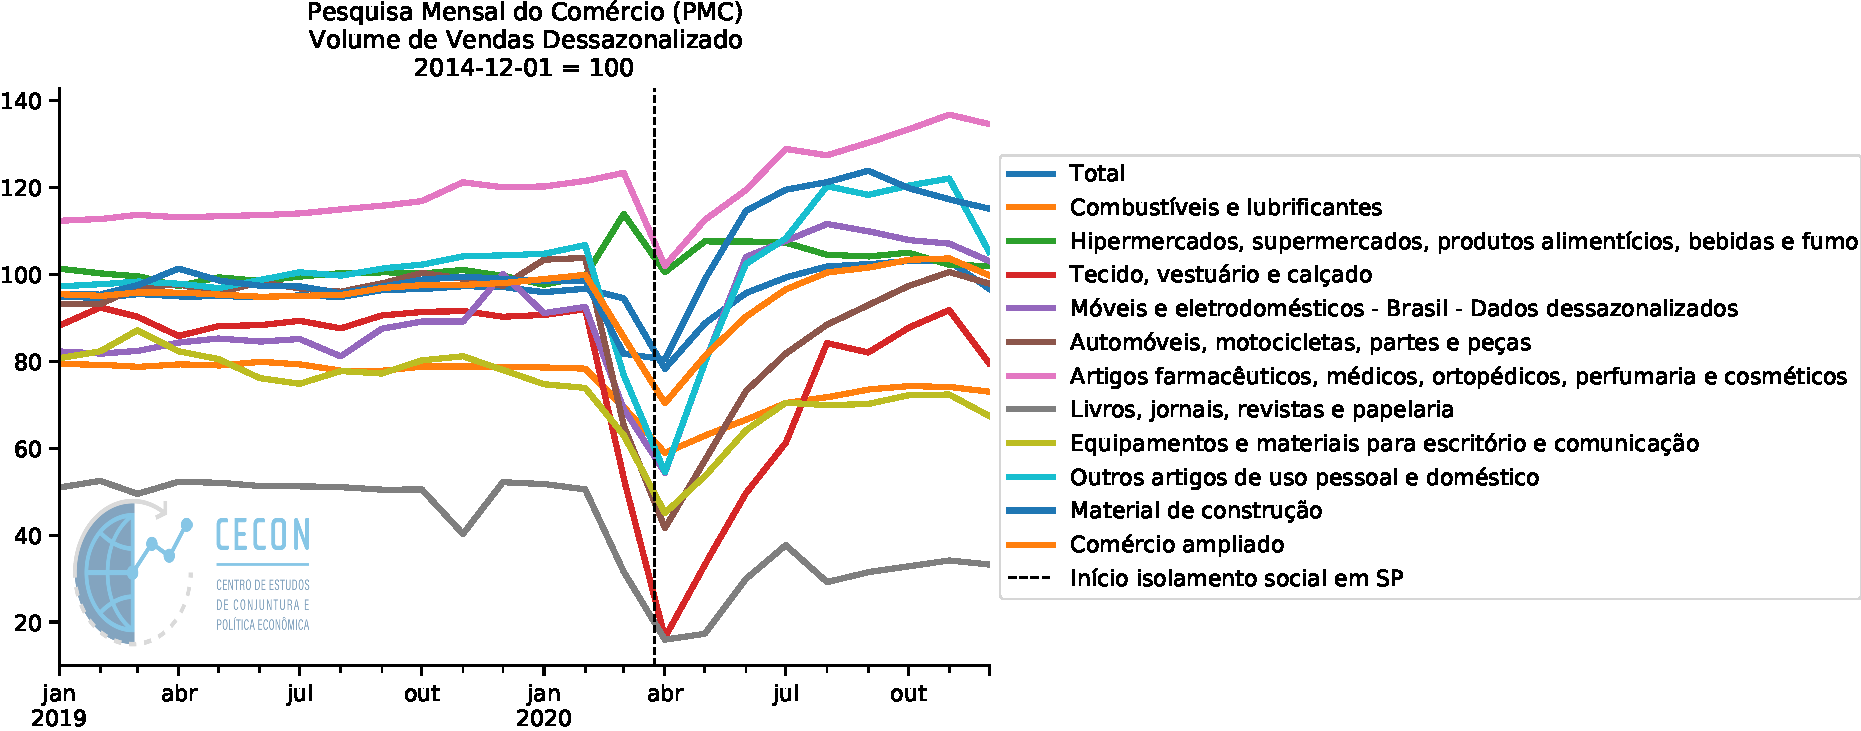
\includegraphics[width=.9\linewidth]{./figs/Setoriais/PMC_IBGE.pdf}
\end{center}


\subsection*{Pesquisa Industrial Mensal (PIM)}
\label{sec:org9725895}

\begin{center}
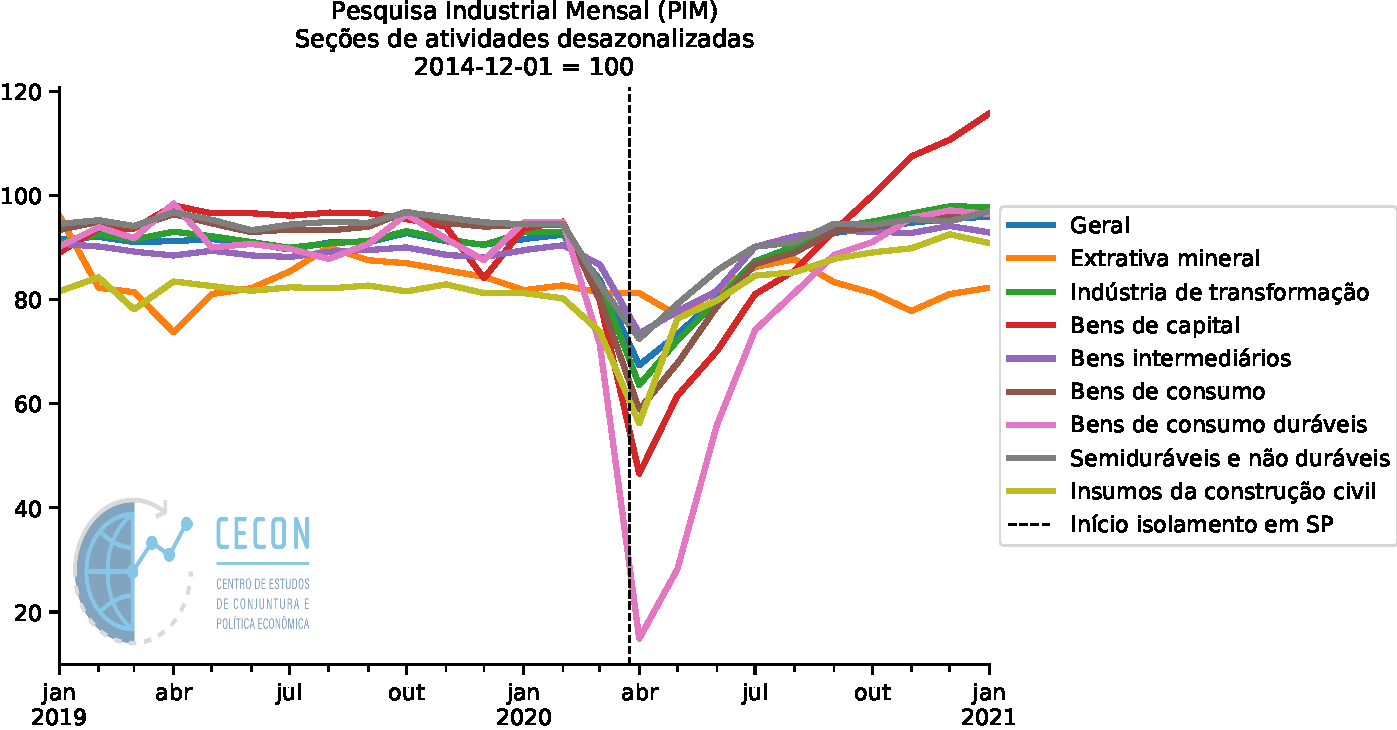
\includegraphics[width=.9\linewidth]{./figs/Setoriais/PIM_IBGE.pdf}
\end{center}


\subsection*{Pesquisa Mensal de Serviços (PMS)}
\label{sec:orgaa5c229}
\subsubsection*{Receita nominal sem ajuste sazonal}
\label{sec:org5916131}
\begin{center}
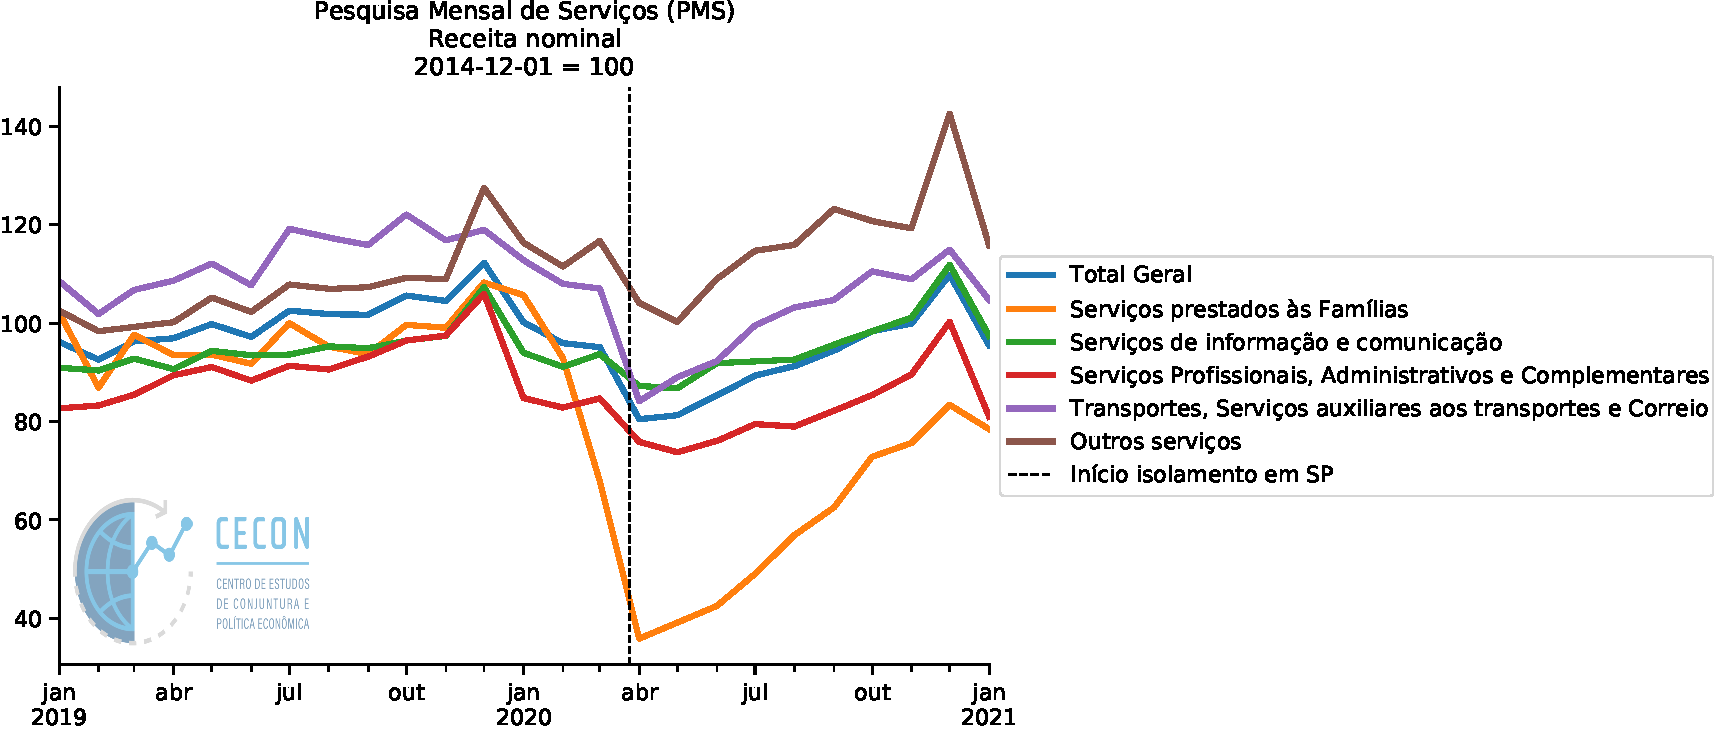
\includegraphics[width=.9\linewidth]{./figs/Setoriais/PMS_IBGE.pdf}
\end{center}

\subsubsection*{Volume com ajuste sazonal}
\label{sec:orgde7e69b}


\begin{center}
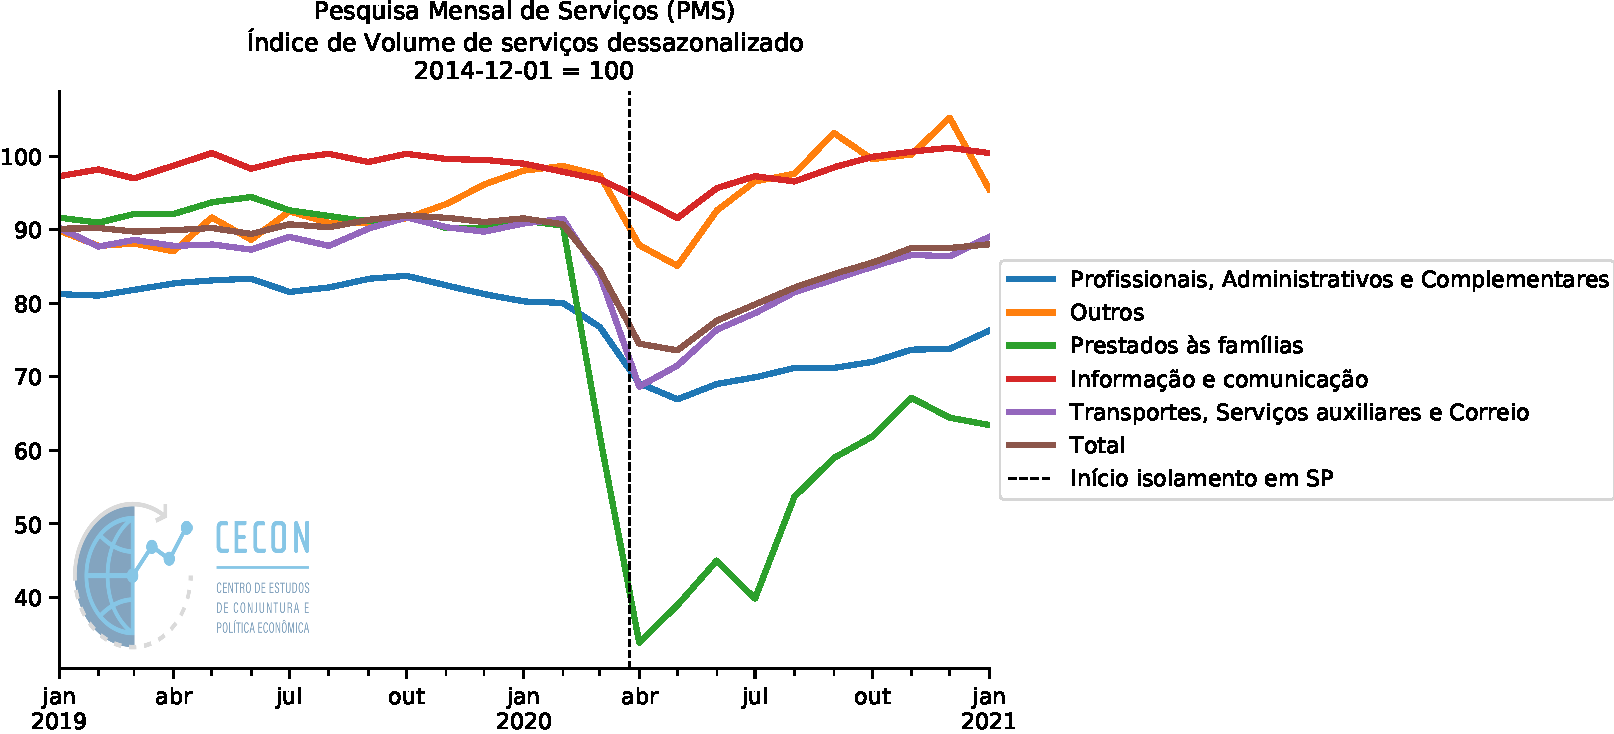
\includegraphics[width=.9\linewidth]{./figs/Setoriais/PMS_vol_dessazonalizada.pdf}
\end{center}

\subsubsection*{Volume com ajuste sazonal (em relação ao mês anterior)}
\label{sec:orgc085c49}


\begin{center}
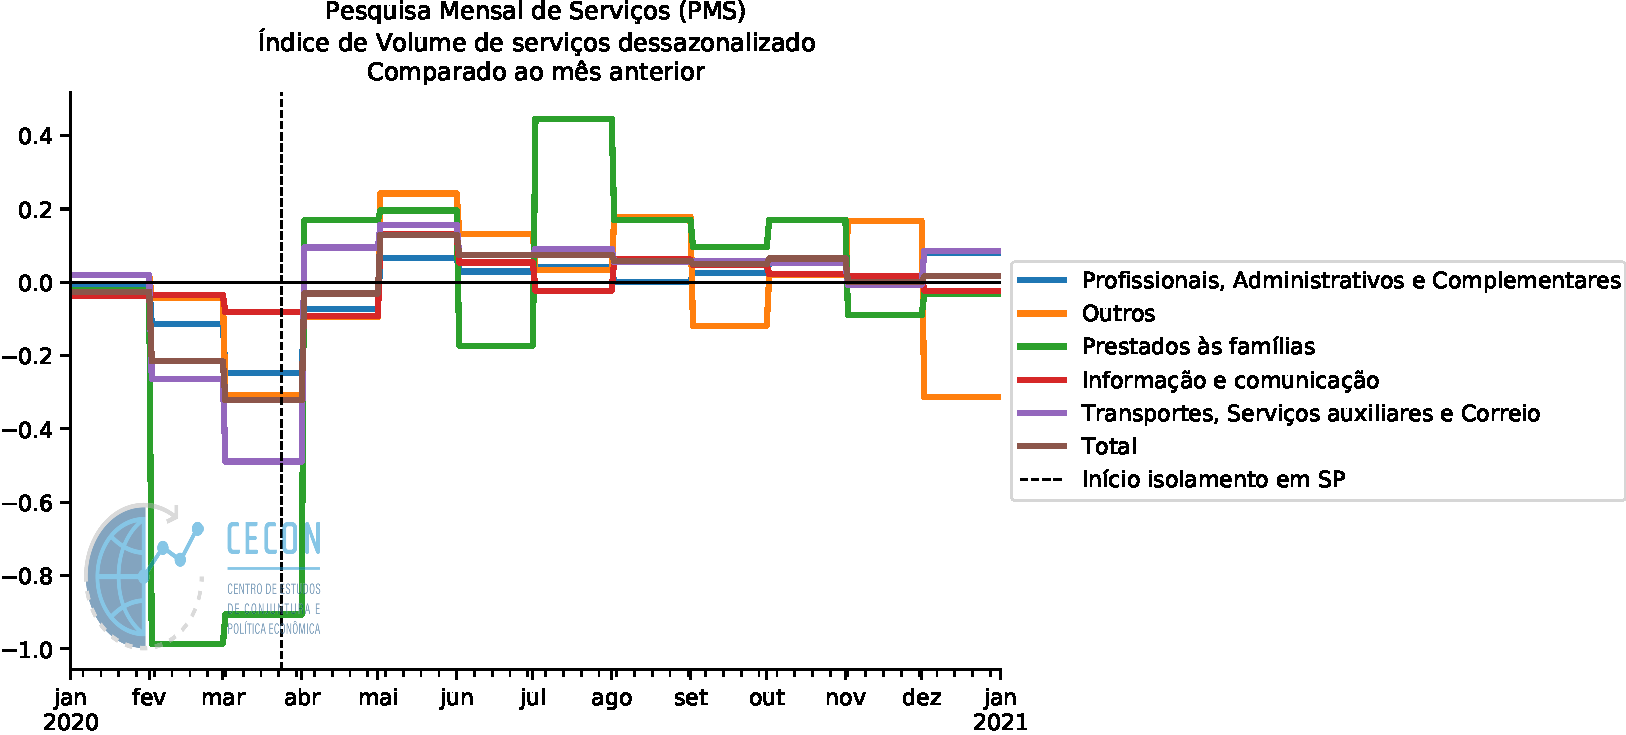
\includegraphics[width=.9\linewidth]{./figs/Setoriais/PMS_vol_dessazonalizada_diff.pdf}
\end{center}

\section*{Emprego}
\label{sec:org04a88d0}

\subsection*{Rendimento médio real habitual das pessoas ocupadas}
\label{sec:org7463d62}


\begin{center}
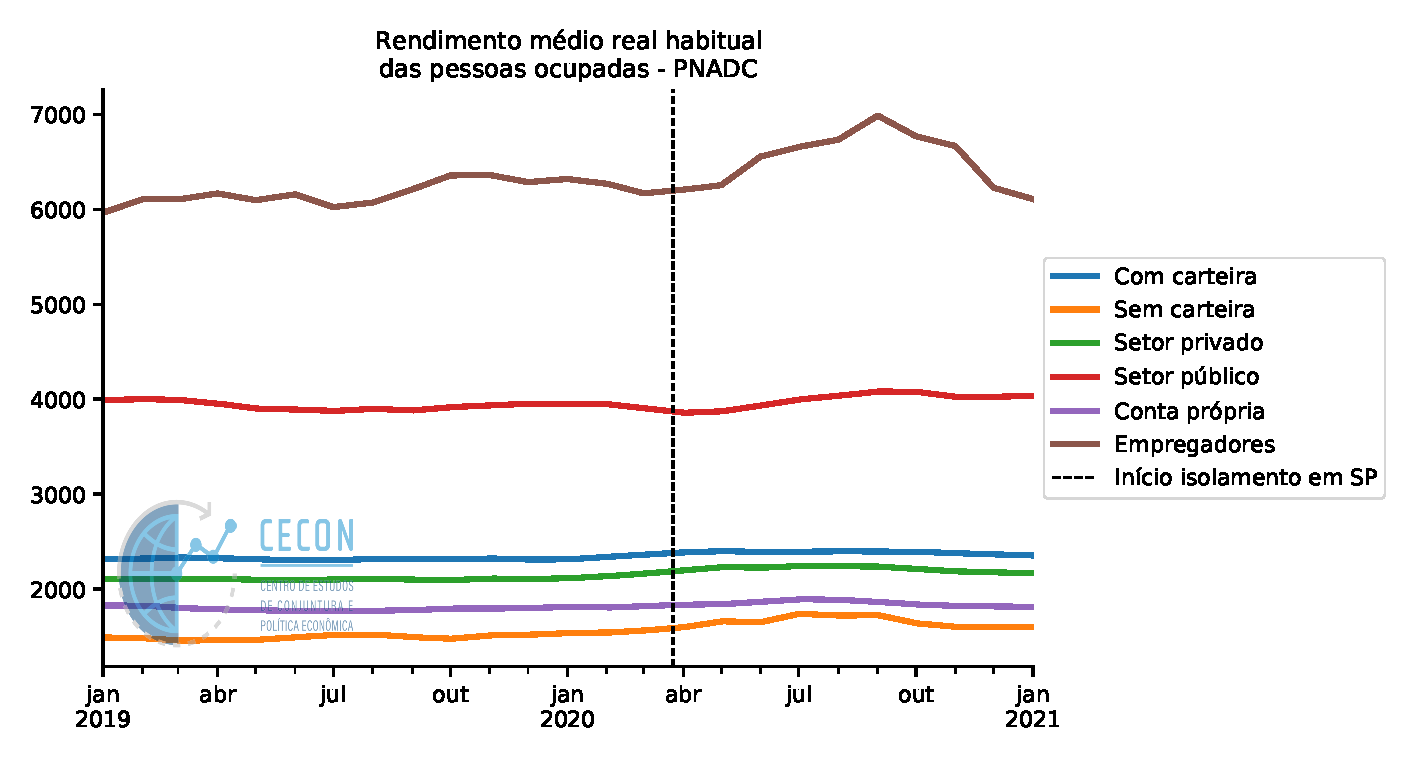
\includegraphics[width=.9\linewidth]{./figs/Emprego/RMHPO.pdf}
\end{center}

\subsection*{Massa de rendimento real efetiva e habitual de todos os trabalhos}
\label{sec:org96d2e68}

\begin{center}
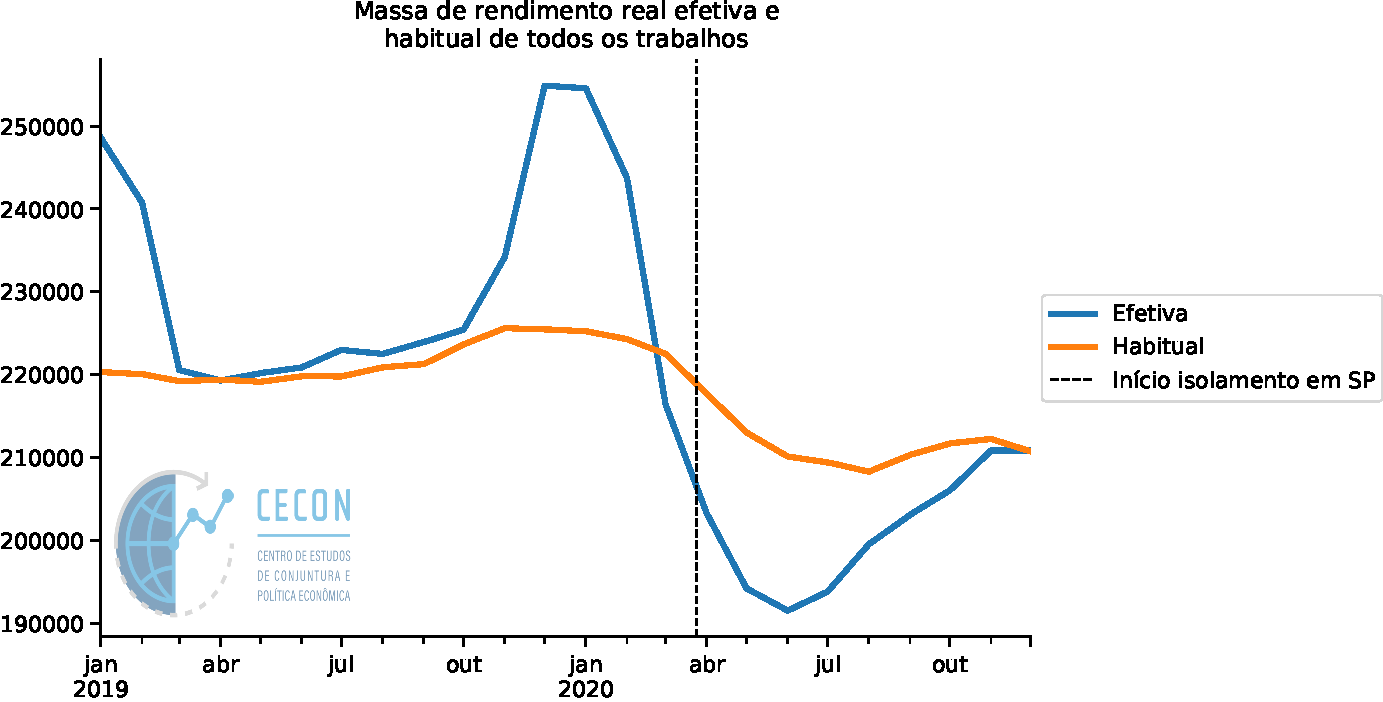
\includegraphics[width=.9\linewidth]{./figs/Emprego/MRR_Efetiva_Habitual.pdf}
\end{center}

\subsection*{Massa Salarial Ampliada Disponível - PNADC}
\label{sec:orgb684d47}

\begin{center}
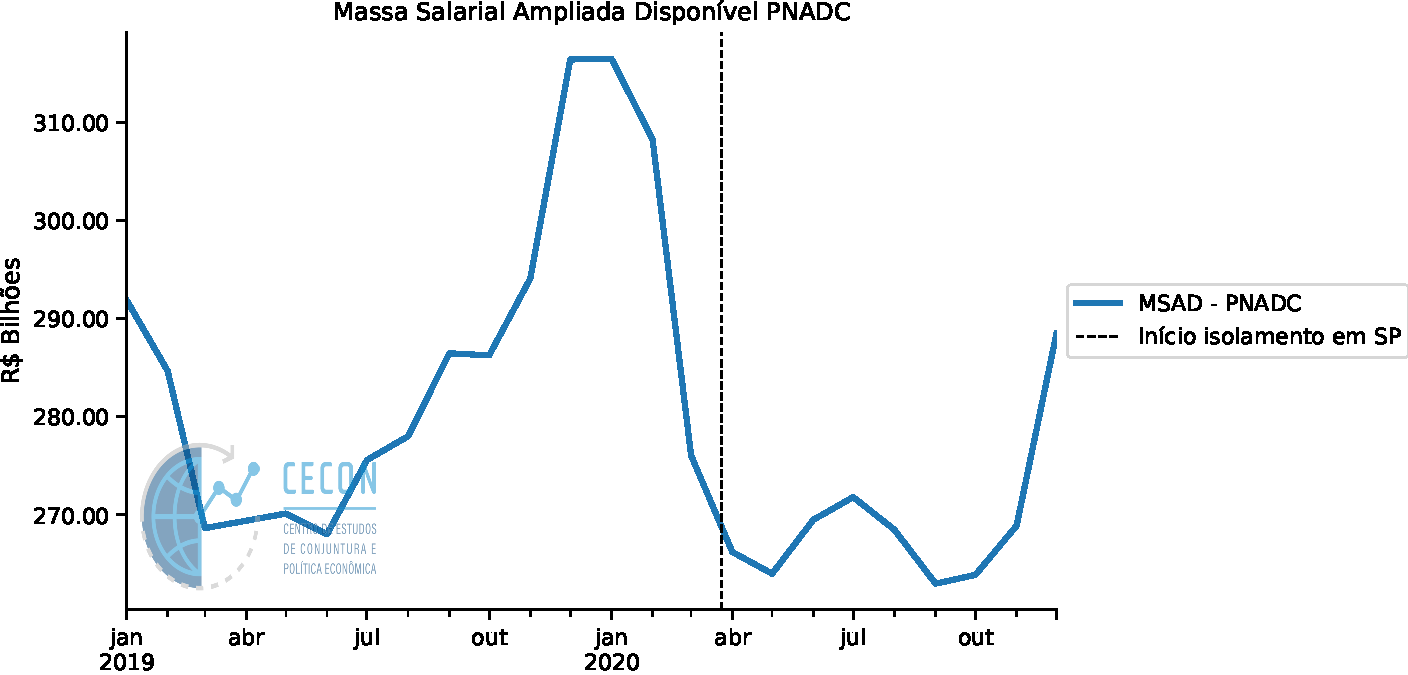
\includegraphics[width=.9\linewidth]{./figs/Emprego/MSAD.pdf}
\end{center}

\subsection*{Rendimento habitual médio por atividade}
\label{sec:orgcac5172}

\subsection*{Número de horas trabalhadas - indústria de transformação}
\label{sec:org90668f7}

\begin{center}
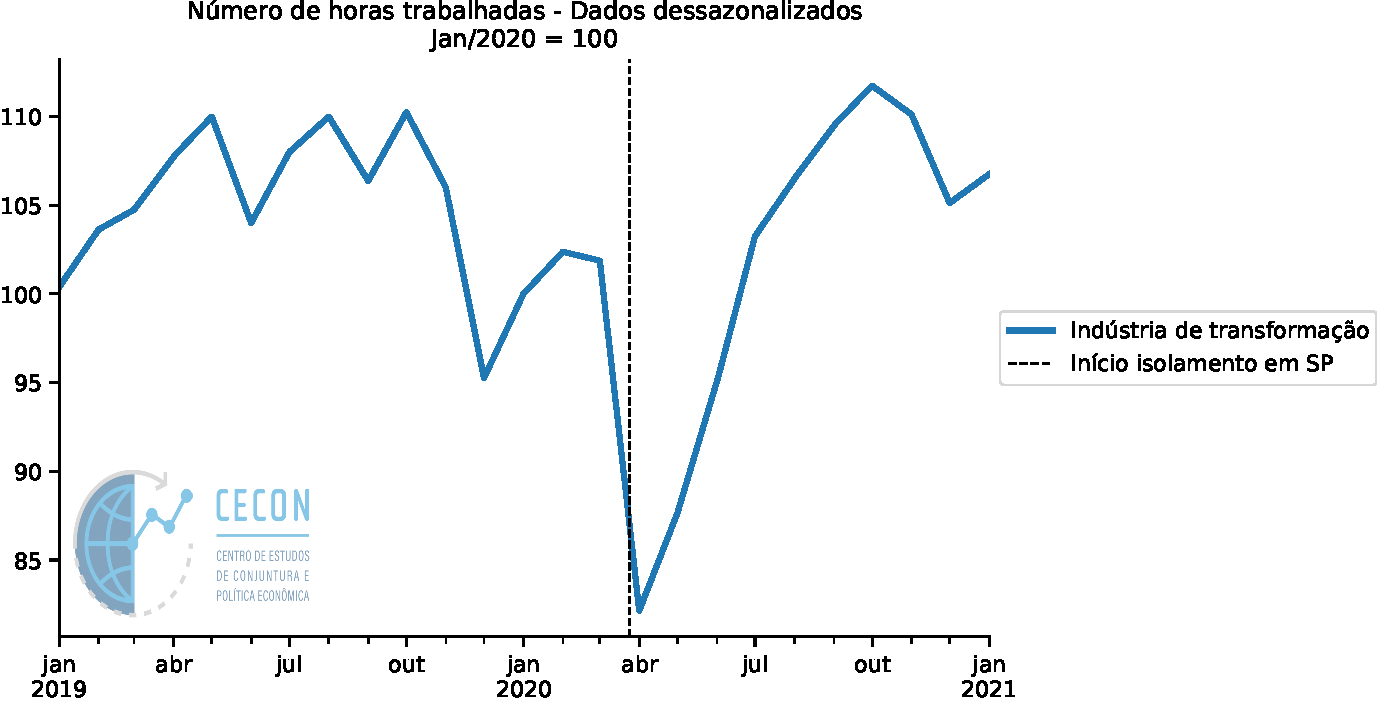
\includegraphics[width=.9\linewidth]{./figs/Emprego/Horas_Transformacao.pdf}
\end{center}

\subsection*{Novo CAGED  - Por atividade (dados dessazonalizados)}
\label{sec:org8666e76}

\begin{center}
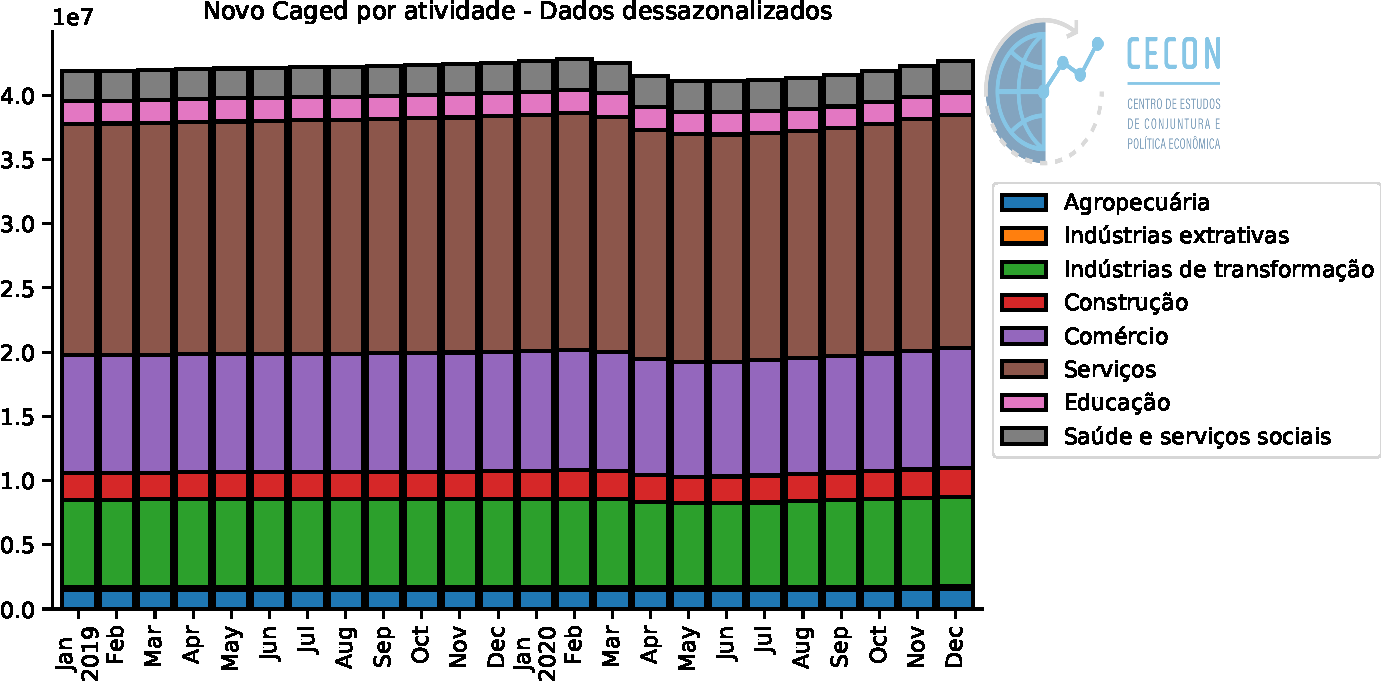
\includegraphics[width=.9\linewidth]{./figs/Emprego/NovoCaged_Atividade.pdf}
\end{center}



\subsection*{Taxa de desocupação}
\label{sec:org6b6bb86}

\begin{center}
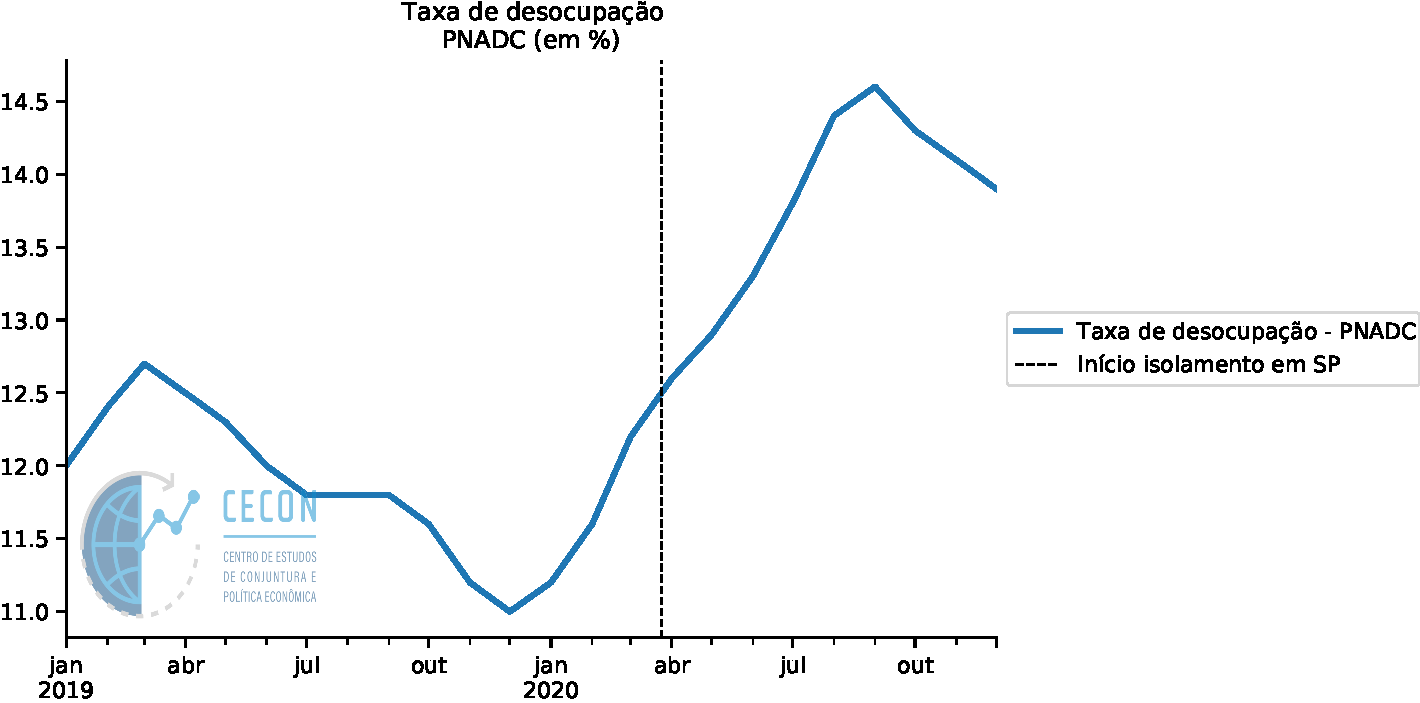
\includegraphics[width=.9\linewidth]{./figs/Emprego/TaxaDesocupacao.pdf}
\end{center}

\section*{PNAD-COVID}
\label{sec:orgaff8a03}
\subsection*{R trial}
\label{sec:org2c2ea83}
\subsection*{Home office - Por sexo e cor}
\label{sec:org5e5da2a}




\begin{center}
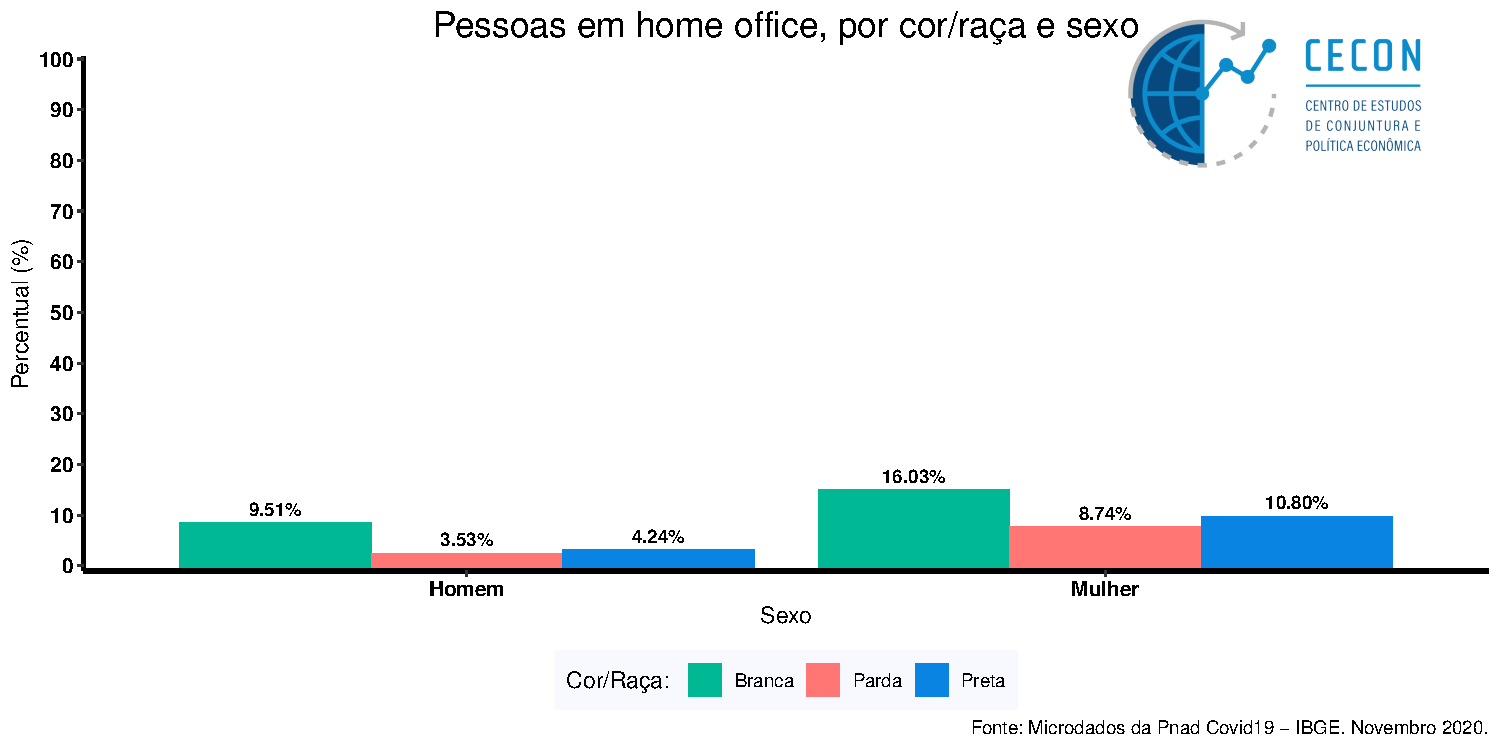
\includegraphics[width=.9\linewidth]{./figs/PNAD_COVID/home_sexo_cor.pdf}
\end{center}

\subsection*{Home office - Por Cor e Escolaridade}
\label{sec:org1e2c231}
\begin{center}
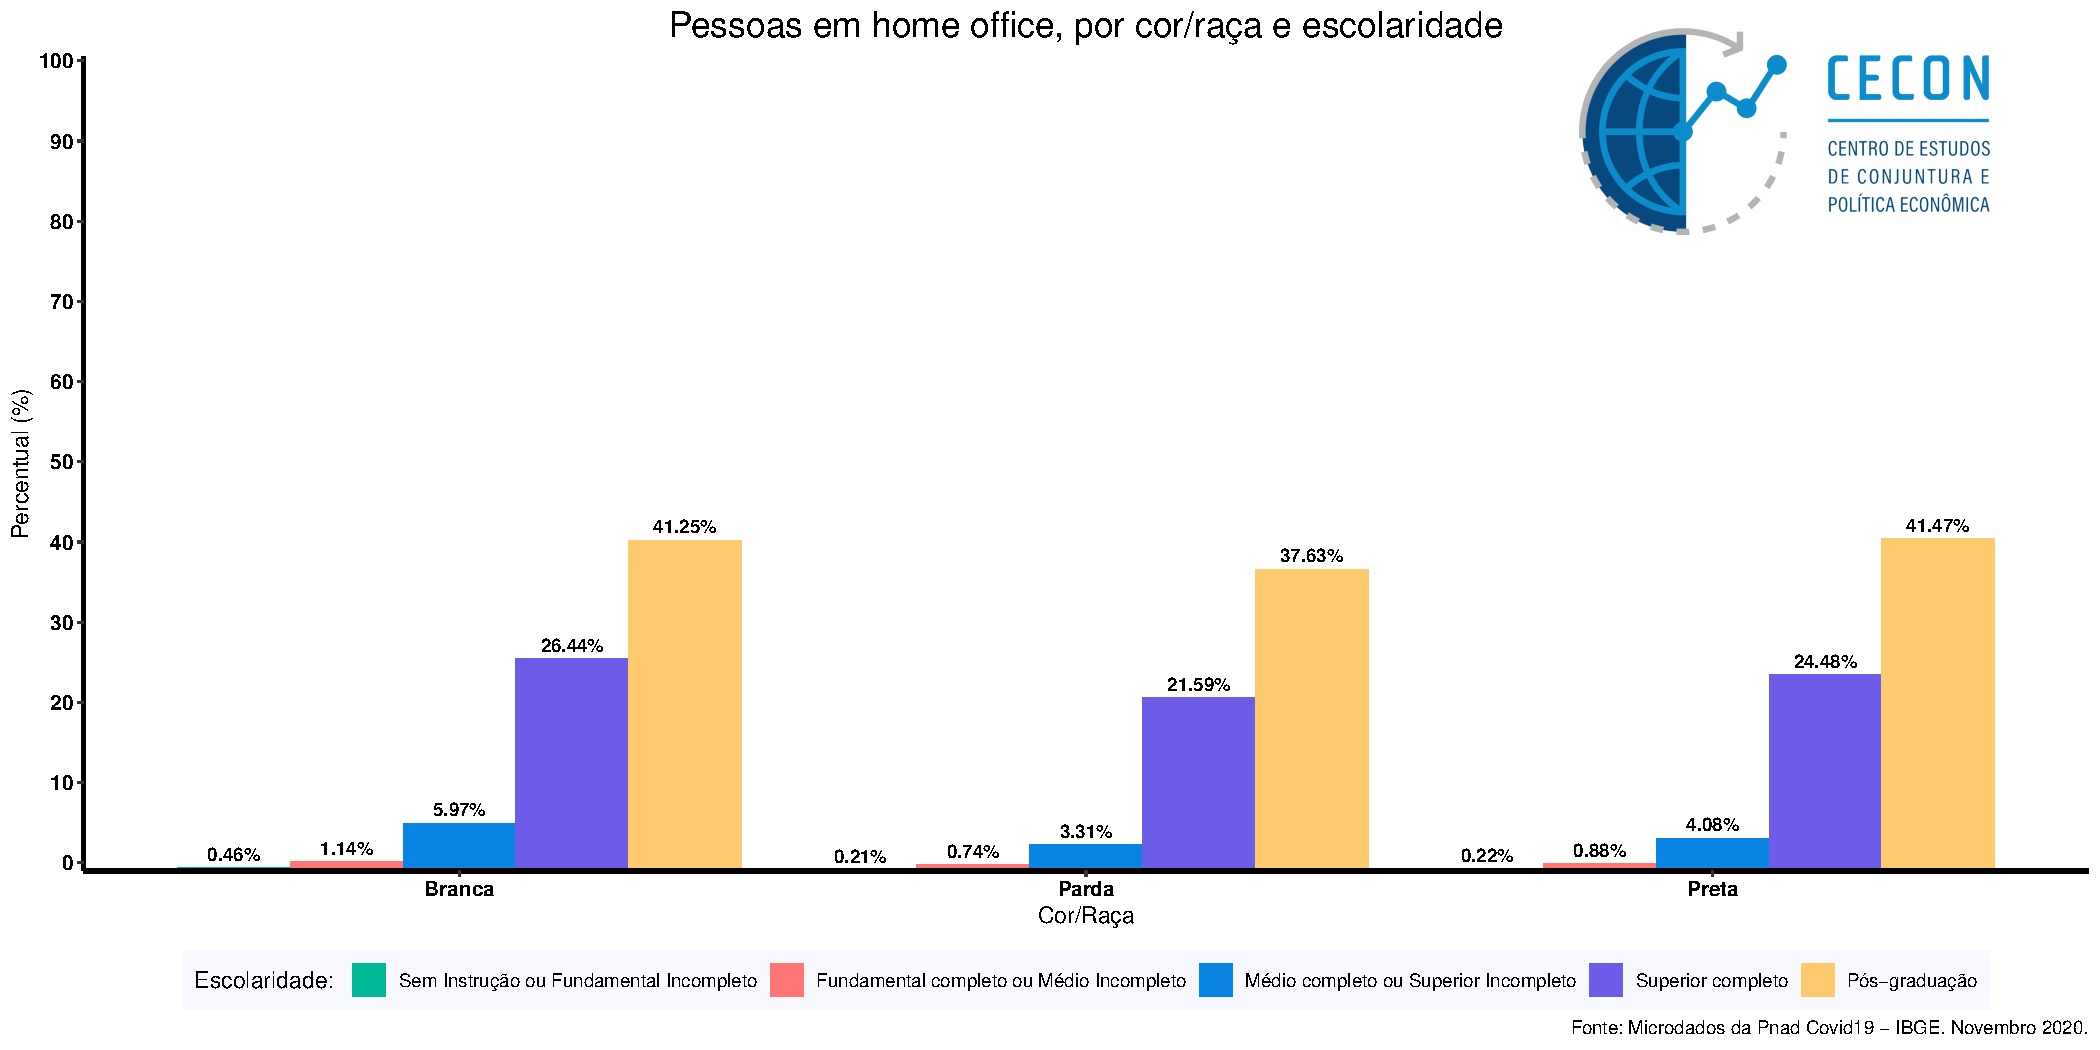
\includegraphics[width=.9\linewidth]{./figs/PNAD_COVID/home_edu_cor.pdf}
\end{center}
\subsection*{Home office - Por Cor e Idade}
\label{sec:org41fe8be}
\begin{center}
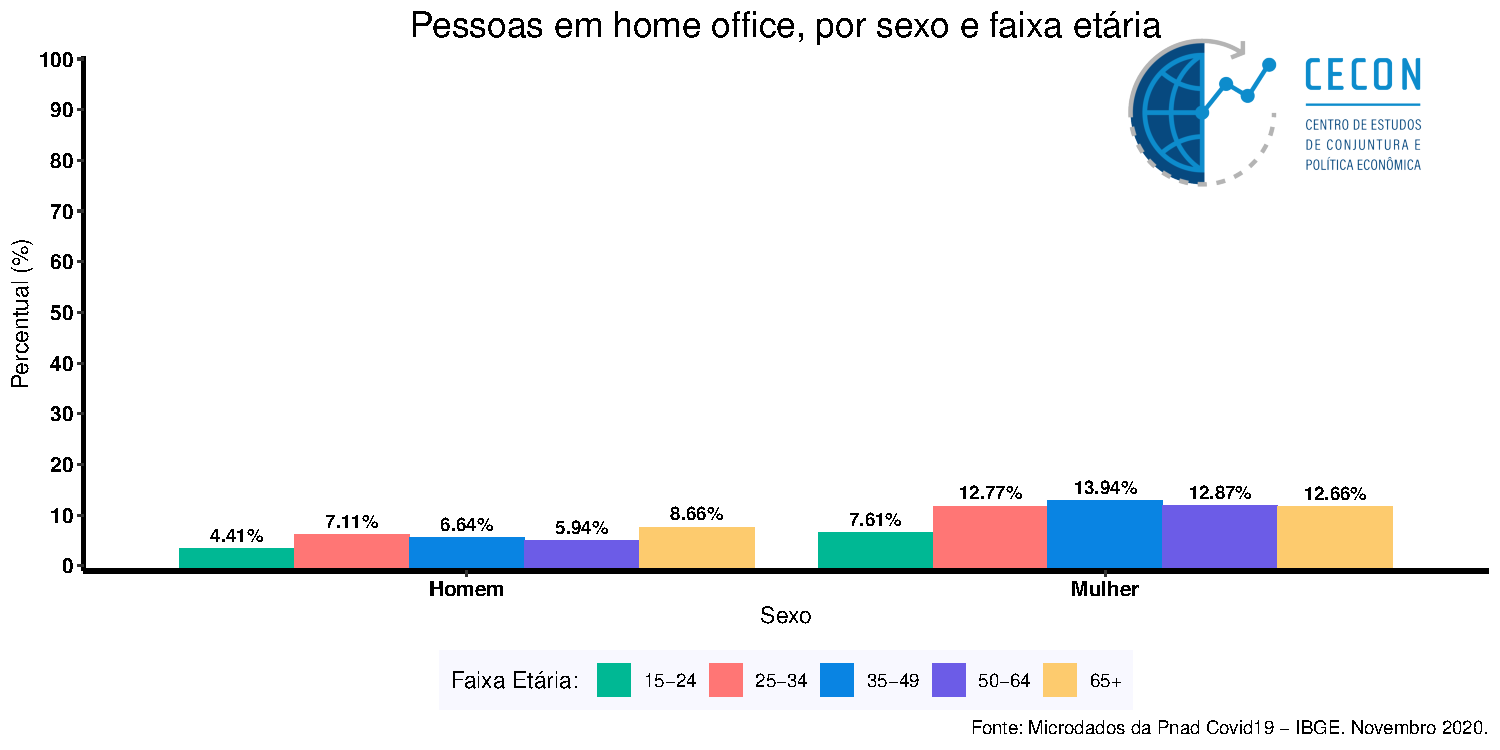
\includegraphics[width=.9\linewidth]{./figs/PNAD_COVID/home_sexo_idade.pdf}
\end{center}

\subsection*{Home office - Por Trabalho}
\label{sec:org0157a7c}
\begin{center}
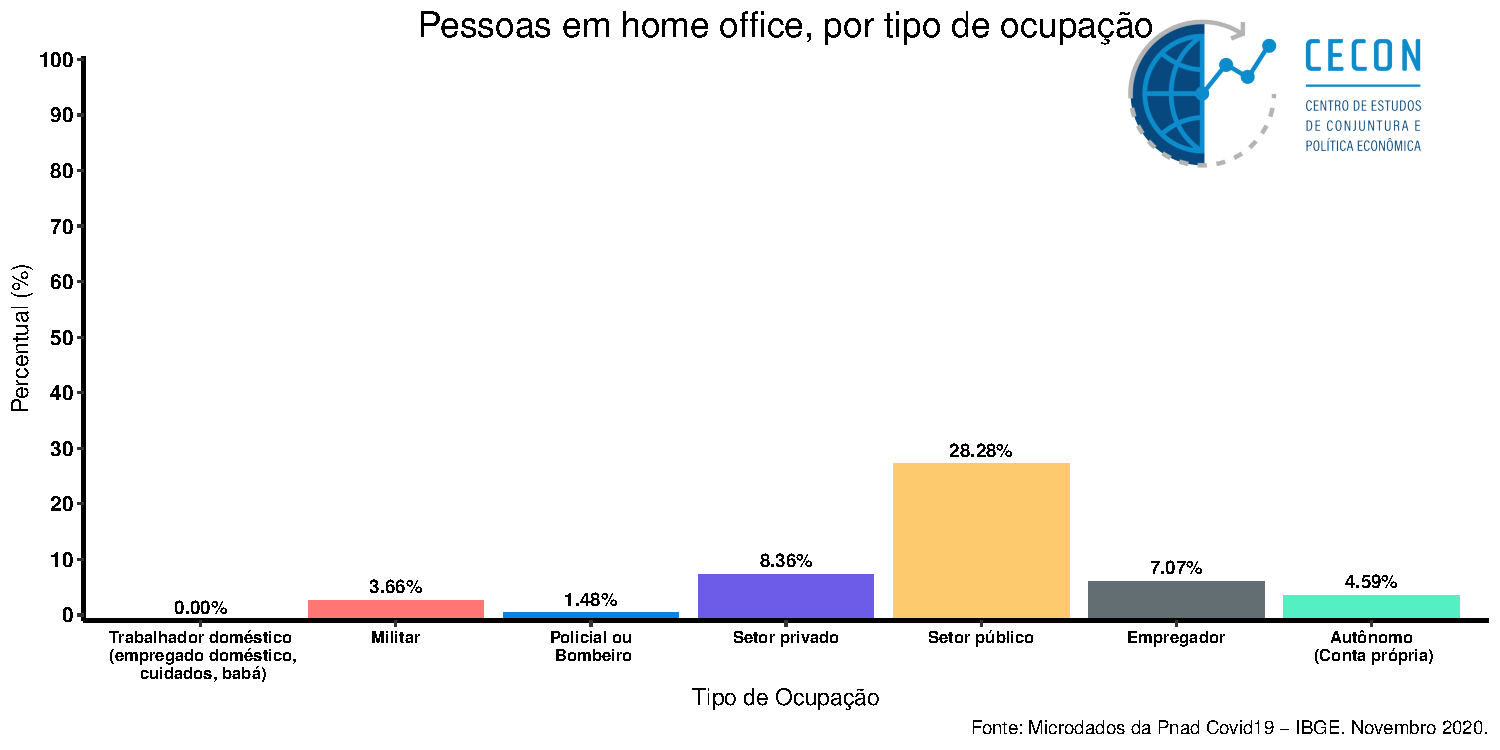
\includegraphics[width=.9\linewidth]{./figs/PNAD_COVID/home_emprego.pdf}
\end{center}

\subsection*{Home office - Por faixa salarial e cor}
\label{sec:orgd2f1848}
\begin{center}
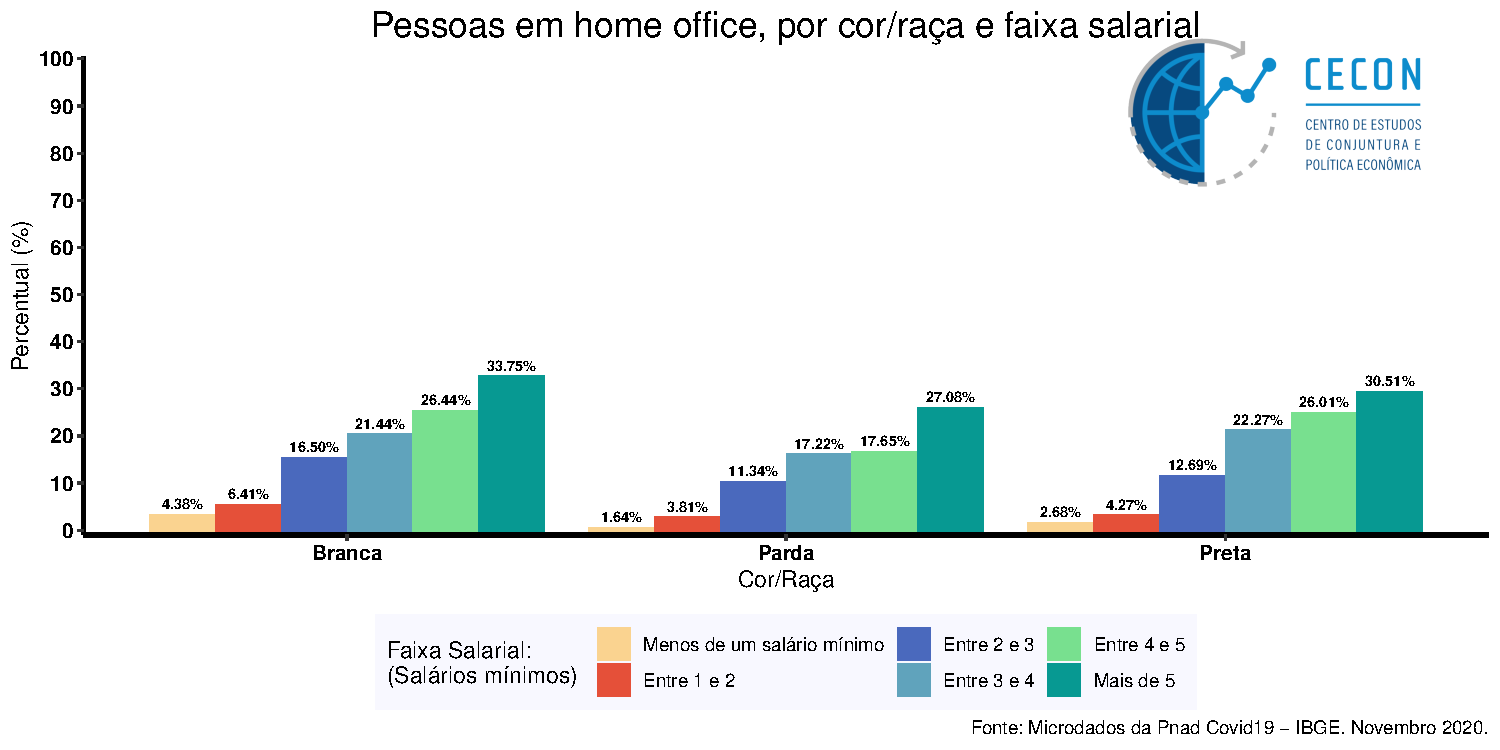
\includegraphics[width=.9\linewidth]{./figs/PNAD_COVID/home_renda.pdf}
\end{center}
\subsection*{Auxilio - Faixa Salarial}
\label{sec:orgafaef69}
\begin{center}
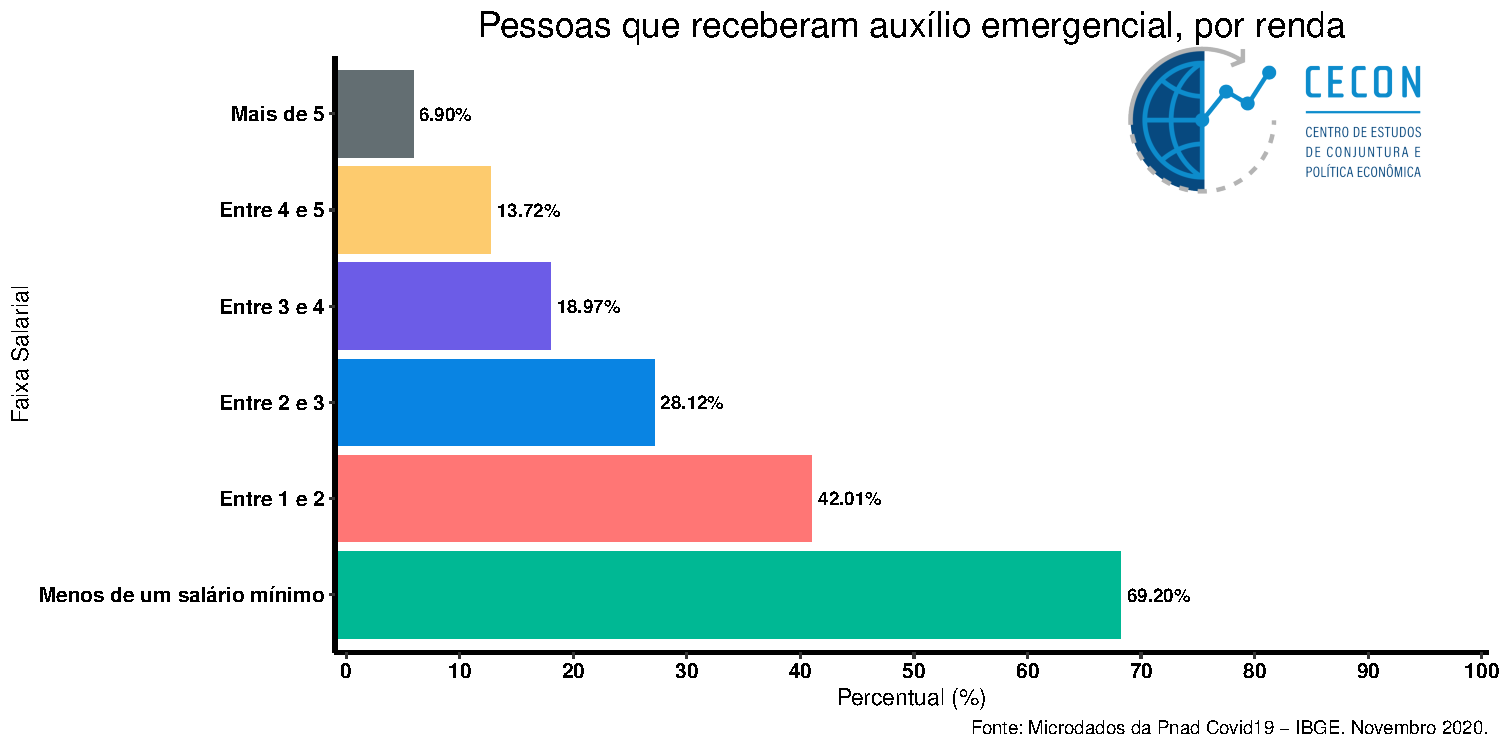
\includegraphics[width=.9\linewidth]{./figs/PNAD_COVID/auxilio_renda.pdf}
\end{center}
\subsection*{Auxilio - Por tipo do domicilio}
\label{sec:org9959cd9}
\begin{center}
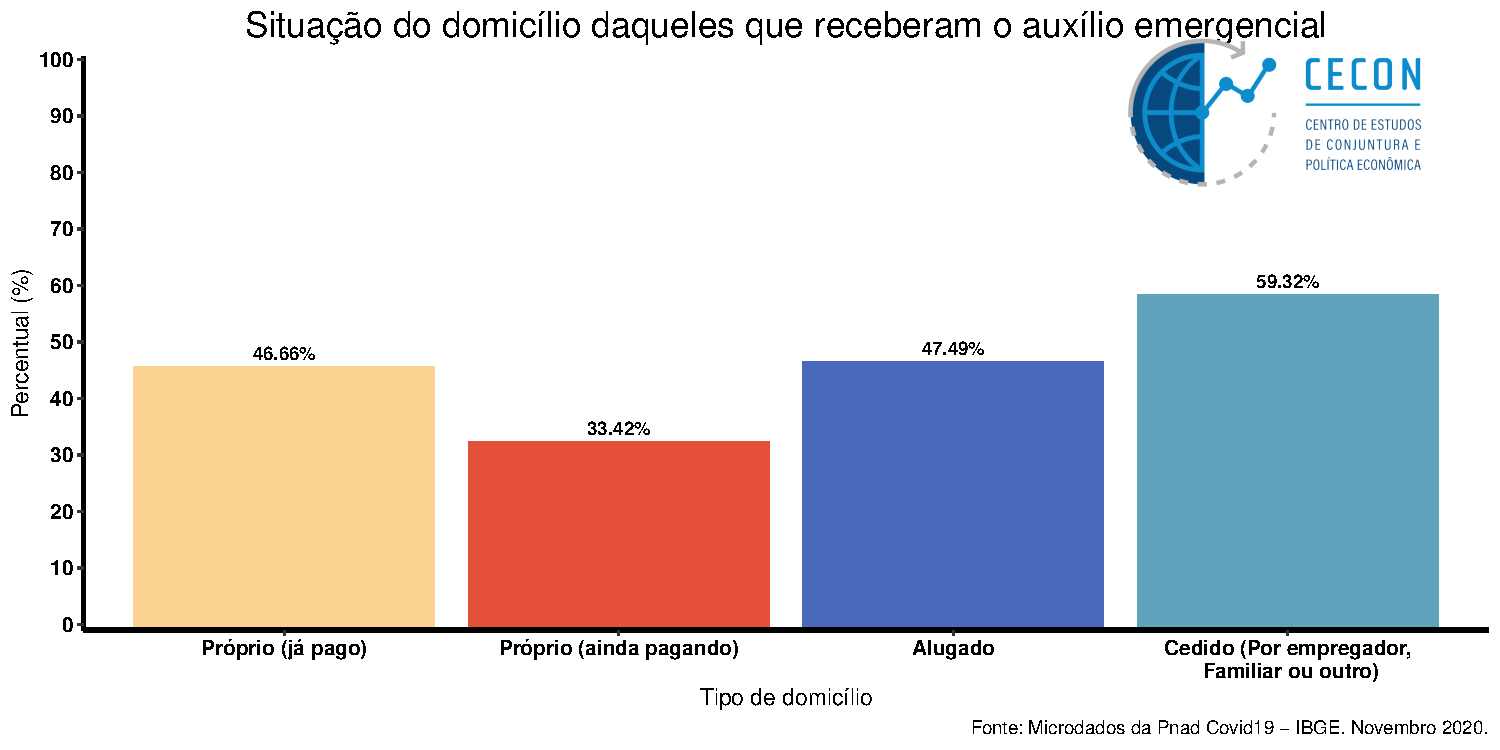
\includegraphics[width=.9\linewidth]{./figs/PNAD_COVID/auxilio_domicilio.pdf}
\end{center}
\subsection*{Auxilio - Sexo e Cor}
\label{sec:org2cfed94}
\begin{center}
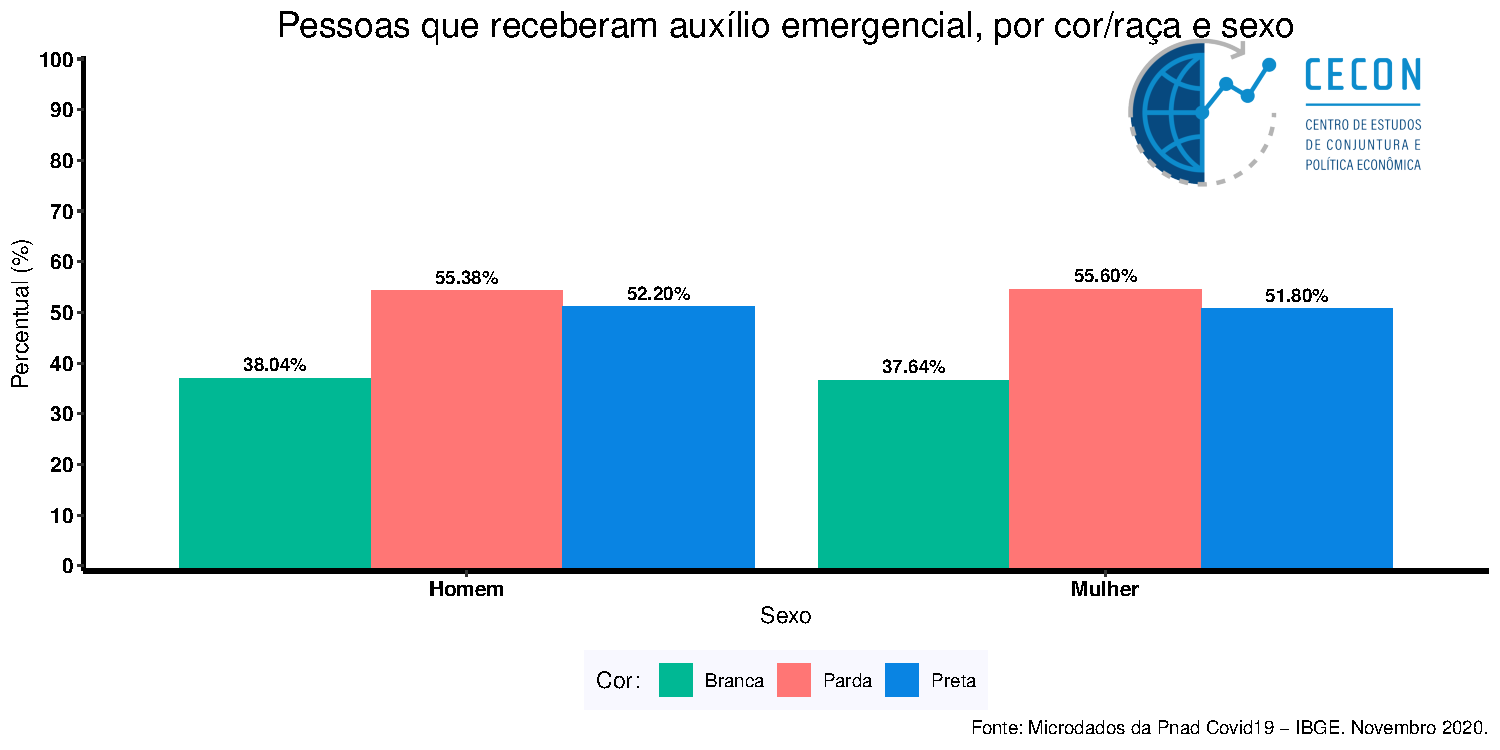
\includegraphics[width=.9\linewidth]{./figs/PNAD_COVID/auxilio_cor_sexo.pdf}
\end{center}


\section*{IMF Fiscal Monitor}
\label{sec:org95b7fa7}
\subsection*{Medidas fiscais em \% do PIB}
\label{sec:orgfe6d707}

\begin{center}
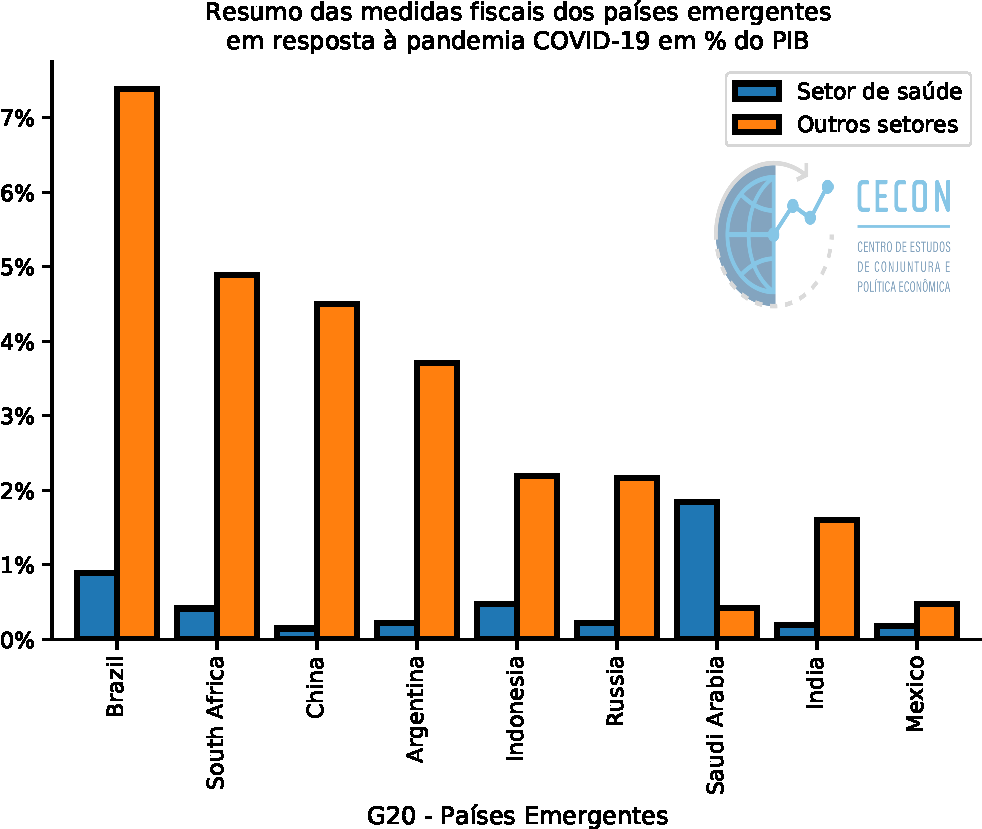
\includegraphics[width=.9\linewidth]{./figs/IMF/FiscalMonitor_Covid.pdf}
\end{center}

\subsection*{Medidas fiscais em \% do PIB: Setor de saúde/Outros setores}
\label{sec:org8098bf6}

\begin{center}
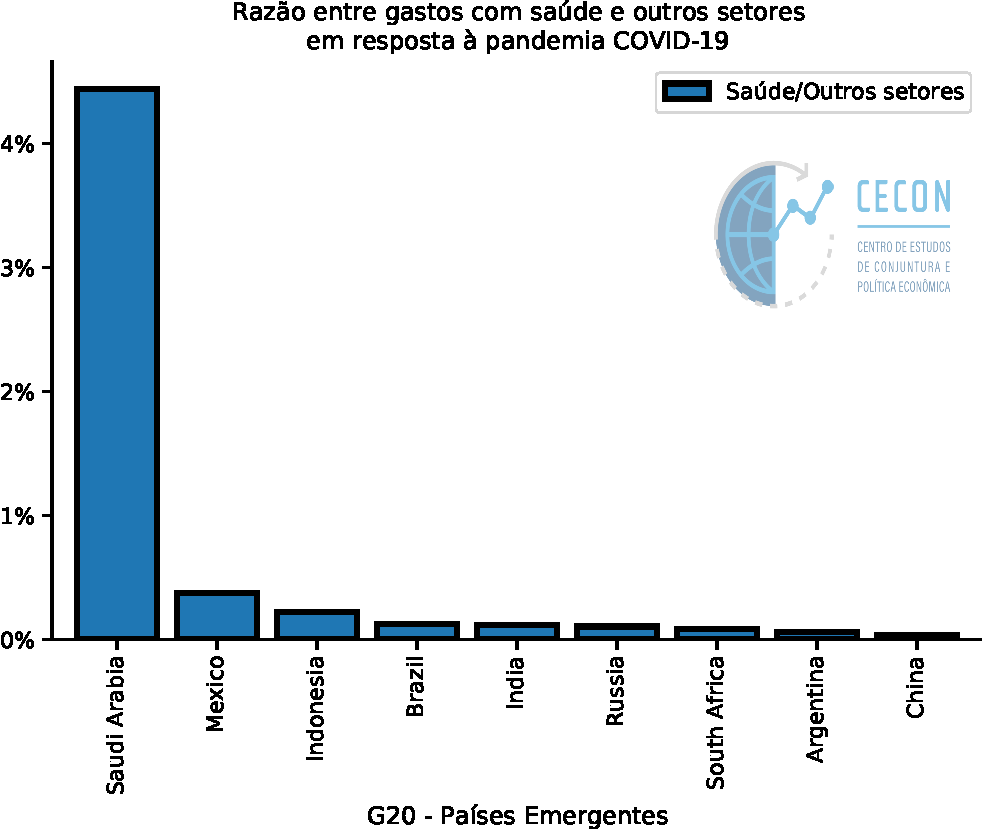
\includegraphics[width=.9\linewidth]{./figs/IMF/FiscalMonitor_Covid_ratio.pdf}
\end{center}

\subsection*{Medidas fiscais em \% do PIB: Setor de saúde/Total}
\label{sec:org41d42b1}

\begin{center}
\includegraphics[width=.9\linewidth]{./figs/IMF/FiscalMonitor_Covid_total.pdf}
\end{center}

\section*{World Economic outlook}
\label{sec:org2904d28}


\subsection*{GDP vs Lockdown}
\label{sec:org5e17b8a}
\begin{table}[htbp]
\caption{\label{IMF_fig_1}GDP Forecast Errors in 2020:H1 and Lockdown Stringency}
\centering
\begin{tabular}{lll}
\hline
Country & GDP Forecast Error & Lockdown Stringency\\
\hline
AUS & -4,54 & 37,21\\
AUT & -9,11 & 37,13\\
BEL & -9,65 & 41,34\\
BRA & -8,71 & 44,01\\
CAN & -8,81 & 40,92\\
CHL & -5,71 & 41,76\\
CHN & -7,82 & 62,36\\
COL & -10,70 & 49,59\\
HRV & -9,36 & 40,25\\
CZE & -8,87 & 34,38\\
DNK & -6,03 & 39,22\\
EST & -6,54 & 31,58\\
FIN & -5,24 & 28,49\\
FRA & -13,44 & 48,72\\
DEU & -7,04 & 35,39\\
GRC & -10,79 & 39,91\\
HKG & -4,45 & 43,62\\
HUN & -8,91 & 38,69\\
IND & -15,70 & 51,69\\
IDN & -6,09 & 42,06\\
IRL & -3,48 & 45,59\\
ISR & -6,44 & 49,81\\
ITA & -11,99 & 51,65\\
JPN & -6,27 & 24,21\\
KOR & -3,02 & 39,64\\
LVA & -7,49 & 33,94\\
LTU & -3,51 & 40,30\\
MYS & -12,54 & 40,67\\
MEX & -11,10 & 41,61\\
NLD & -6,49 & 40,82\\
NOR & -6,10 & 32,55\\
PER & -20,54 & 55,43\\
PHL & -15,14 & 58,33\\
POL & -6,56 & 40,53\\
PRT & -10,87 & 43,79\\
ROU & -7,04 & 44,54\\
RUS & -4,29 & 48,61\\
SRB & -4,59 & 40,73\\
SGP & -7,63 & 43,65\\
SVK & -10,39 & 40,44\\
SVN & -11,35 & 34,24\\
ZAF & -9,66 & 47,21\\
ESP & -14,65 & 42,21\\
SWE & -4,28 & 21,08\\
CHE & -6,16 & 37,10\\
TWN & -1,37 & 13,73\\
THA & -9,13 & 39,43\\
TUR & -5,42 & 42,28\\
UKR & -8,08 & 47,94\\
GBR & -12,91 & 38,99\\
USA & -6,44 & 43,14\\
VNM & -4,35 & 47,91\\
\hline
\end{tabular}
\end{table}


\begin{center}
\includegraphics[width=.9\linewidth]{./figs/IMF/GDP_Lockdown.pdf}
\end{center}



\subsection*{Lockdown: Voluntary vs Stringency}
\label{sec:org6996447}

\begin{table}[htbp]
\caption{\label{Vol_String}Impact of Lockdowns and Voluntary Social Distancing on Mobility during the First 90 Days of Each Country’s Epidemic}
\centering
\begin{tabular}{lll}
Country groups & Lockdown stringency & Voluntary social distancing\\
\hline
All & -7,85 & -6,53\\
AEs & -8,07 & -10,62\\
EMs & -8,78 & -6,26\\
LICs & -5,8 & -2,83\\
\hline
\end{tabular}
\end{table}

\begin{center}
\includegraphics[width=.9\linewidth]{./figs/IMF/Vol_String.pdf}
\end{center}

\subsection*{Sequencing of lockdown measures}
\label{sec:org5aead0a}
\begin{table}[htbp]
\caption{\label{Lock_measure}Sequencing of lockdown measures}
\centering
\begin{tabular}{lrrr}
\hline
Lockdown measures & Middle & Low & High\\
\hline
Stay-at-home orders & 18 & 10 & 27\\
Public transport closures & 16 & 7,5 & 25\\
Internal movement restrictions & 16 & 7 & 27\\
Workplace closures & 13 & 6 & 22\\
Gathering restrictions & 10 & 2 & 20\\
Public event cancellations & 6 & 1 & 14,5\\
School closures & 4,5 & 1 & 13,5\\
International travel controls & 1 & 0 & 9\\
\hline
\end{tabular}
\end{table}

\begin{center}
\includegraphics[width=.9\linewidth]{./figs/IMF/Lock_measures.pdf}
\end{center}

\section*{OECD Weekly tracker}
\label{sec:org31fbc9f}

\begin{center}
\includegraphics[width=.9\linewidth]{./figs/Granulares/OCDE_Semanal.pdf}
\end{center}

\subsection*{Informações adicionais}
\label{sec:org4d119c0}

Conforme sugere o Anexo A (p. 40) de \textcite{woloszko_2020_Tracking}, a semana considerada se inicia aos domingos.
Compara-se com a mesma semana do ano anterior cujos dias da semana são os mais próximos da data de referência do ano corrente.
Exemplo dado pelo autor (p. 43):

\begin{quote}
The log difference for, say, 03-01-2020, is obtained by taking the difference between the \(svi_{03 −01 −2020}\) and the log of a weighted average of the closest known values before and after 03-01-2019, that is 31-12-2018 and 07-01-2019.
\end{quote}


\section*{Auxílio emergencial}
\label{sec:org69d7889}

\npdecimalsign{,}
\npthousandsep{.}
\nprounddigits{0}
\begin{figure}[h]
    \resizebox{\textwidth}{!}{%
    \begin{tabular}{l|n{5}{2}|n{5}{2}|n{5}{2}|n{5}{2}|n{5}{2}|n{5}{2}|n{5}{2}|n{5}{2}|n{5}{2}|n{5}{2}|n{5}{2}}
\hline\hline
\multirow{2}{*}{(R\$ em milhões)} &
  \multicolumn{5}{c|}{Auxílio Emergencial} &
  \multicolumn{4}{c|}{Extensão do Auxílio Emergencial} &
  \multicolumn{1}{c|}{\multirow{2}{*}{2020}} &
  \multicolumn{1}{c}{\multirow{2}{*}{\% PIB 2020}} \\\cline{2-10}
 &
  \multicolumn{1}{c|}{abr/20} &
  \multicolumn{1}{c|}{mai/20} &
  \multicolumn{1}{c|}{jun/20} &
  \multicolumn{1}{c|}{jul/20} &
  \multicolumn{1}{c|}{ago/20} &
  \multicolumn{1}{c|}{set/20} &
  \multicolumn{1}{c|}{out/20} &
  \multicolumn{1}{c|}{nov/20} &
  \multicolumn{1}{c|}{dez/20} &
  \multicolumn{1}{c|}{} &
  \multicolumn{1}{c}{} \\\hline
AE Total &
  35781,054122 &
  41187,560652 &
  44699,80172948 &
  45919,51720376 &
  45060,964856 &
  24001,64923417 &
  20896,05343287 &
  18522,98326748 &
  18496,42121275 &
  294566,00571051 &
  4,0 \\
AE PBF &
  15176,3958 &
  15200,424 &
  15217,0812 &
  15141,69 &
  15196,3308 &
  4494,105196 &
  4380,11041 &
  4315,80209145 &
  4267,628712 &
  93389,56820945 &
  1,3 \\
AE CadÚnico não PBF &
  7018,7244 &
  6951,8544 &
  6619,3056 &
  6610,6482 &
  6368,0328 &
  2920,1895 &
  2863,8336 &
  2830,8507 &
  2801,0811 &
  44984,5203 &
  0,6 \\
AE Aplicativo &
  13585,7946 &
  19035,1344 &
  22859,7522 &
  24158,1816 &
  23456,7612 &
  16553,6688 &
  13623,9447 &
  11355,6693 &
  11411,8881 &
  156040,7949 &
  2,1 \\
AE Judicial &
  0,0954 &
  0,1039 &
  3,61874648 &
  8,95339076 &
  39,796012 &
  33,64166317 &
  28,12061787 &
  20,61704003 &
  15,77913475 &
  150,72590506 &
  0,0 \\
 &
   &
   &
   &
   &
   &
   &
   &
   &
   &
   &
   \\
PBF 2019 abril a dezembro &
  2632,27853599999 &
  2677,539162 &
  2627,861441 &
  2609,28159000001 &
  2608,191765 &
  2561,39384200001 &
  2564,19320299999 &
  2520,210959 &
  2525,74600700001 &
  23327 &
   \\
PBF 2019 para 2020 &
   &
   &
   &
   &
   &
   &
   &
   &
   &
  24381 &
   \\
 &
   &
   &
   &
   &
   &
   &
   &
   &
   &
   &
   \\
``AE efetivo'' (sem despesa de PBF) &
   &
   &
   &
   &
   &
   &
   &
   &
   &
  270185 &
  3,6 \\
 &
   &
   &
   &
   &
   &
   &
   &
   &
   &
   &
   \\
Valor 2021 &
   &
   &
   &
   &
   &
   &
   &
   &
   &
  44000 &
  0,6 \\
Equivalente a set/out. 2020 &
   &
   &
   &
   &
   &
   &
   &
   &
   &
  44898 &\\\hline\hline
\end{tabular}

\end{figure}

\section*{Novos casos x Restrição de mobilidade por tipo de isolamento}
\label{sec:orgaf76eae}
\subsection*{Inspeção dos picos}
\label{sec:org5680740}

\begin{center}
\includegraphics[width=.9\linewidth]{./figs/COVID/Picos.pdf}
\end{center}


\subsection*{Descrição dos dados}
\label{sec:org33d16d3}
\begin{longtable}{c|p{2cm}|p{5cm}|p{5cm}|p{3cm}}
\hline
Eixo & Nome & Descrição & Ajuste & Motivo\\
\hline
\endfirsthead
\multicolumn{5}{l}{Continued from previous page} \\
\hline

Eixo & Nome & Descrição & Ajuste & Motivo \\

\hline
\endhead
\hline\multicolumn{5}{r}{Continued on next page} \\
\endfoot
\endlastfoot
\hline
Y & Taxa de crescimento de novos casos & Taxa de crescimento dos novos casos de COVID-19 por milhão de habitantes & Foram removidos casos em que a taxa de crescimento foi acima de 10\% e menor de -10\% em relação ao dia anterior & Remover potenciais outliers\\
\hline
X & Fase da pandemia & Descreve se a pandemia ocorreu antes do primeiro pico após as 5 primeiras mortes; desde o primeiro pico ate o pico da segunda onda e; pós-segunda onda para captar países em que a pandemia não esta controlada. & Se o total de mortes for menor que 100, não será categorizado como pico da respectiva onda. & Não classificar máximos locais em uma janela pequena (menos de 14 dias) como um pico e, por consequência, incluir mais picos do que os existentes.\\
\hline
Cores & Tipo de isolamento & Se o tempo que as pessoas ficaram em casa (em relação à 14 dias atrás) aumentar e não houver medida de restrição no dia, voluntário. Se o tempo que as pessoas ficaram em casa (em relação à 14 dias atrás) aumentar e houver medida de restrição, imposto. Se o tempo que as pessoas ficaram em casa diminuiu, queda. & Foram removidos casos em que a taxa de variação do tempo que as pessoas ficaram em casa for maior que 100\% em módulo. & Para remover possívies outlier. Foi considerada a comparação com 14 dias atrás para evitar efeitos do fim de semana e contemplar situações em que as medidas de restrições não foram de curta duração.\\
\hline
Largura & - & Os boxplots serão tão mais largos quanto mais observações existirem para a fase da pandemia. Assim, um boxplot mais largo no pós-segundo pico indica que exitem mais observaçeõs se comparados com o restante da pandemia. & - & -\\
\hline
Altura & - & Os boxplots serão tão mais altos quanto maior a dispersão nas taxas de crescimento & - & -\\
\hline
\end{longtable}

\subsection*{Novos casos por milhão x Fase pandemia (sem aparar dados)}
\label{sec:org15d532c}
\begin{center}
\includegraphics[width=.9\linewidth]{./figs/COVID/Casos_Policy_Todos.pdf}
\end{center}


\subsection*{Novos casos por milhão x Fase pandemia (mais de 10 casos por milhão de habitante)}
\label{sec:orgee6c86a}

\begin{center}
\includegraphics[width=.9\linewidth]{./figs/COVID/Casos_Policy_10_Todos.pdf}
\end{center}

:results:
\begin{center}
\includegraphics[width=.9\linewidth]{./figs/COVID/Casos_Policy_10_Todos.pdf}
\end{center}
\subsection*{Novos casos por milhão x Fase pandemia (mais de 50 casos por milhão de habitante)}
\label{sec:org2fa1737}

\begin{center}
\includegraphics[width=.9\linewidth]{./figs/COVID/Casos_Policy_50_Todos.pdf}
\end{center}

\subsection*{Novos casos por milhão x Fase pandemia (mais de 100 casos por milhão de habitante)}
\label{sec:org80e6c00}

\begin{center}
\includegraphics[width=.9\linewidth]{./figs/COVID/Casos_Policy_100_Todos.pdf}
\end{center}


\subsection*{Texto explicativo}
\label{sec:org02ec251}

Neste ponto, cabe discutir a relavância do isolamento social voluntário e sua relação com o estágio da pandemia.
Para isso, associa-se o tipo de isolamento social (se voluntário, imposto ou em queda) com as diferentes fases da pandemia e com as taxas de crescimento de novos casos por meio de \emph{boxplots} como indicado pela figura abaixo.
O eixo das coordenadas indica a taxa de crescimento de novos casos por milhão de habitantes e possui uma linha horizontal em zero para facilitar a visualização.
O eixo das abscissas apresenta a respectiva fase da pandemia em casa país.
Denomina-se de ``início ao primeiro pico'' como período em que o número acumulado de mortes é superior à 100 e que a taxa de crescimento de novos casos foi a maior em uma janela de 28 dias\footnote{Mais precisamente, 14 dias depois e antes do dia em questão.}.
A mesma janela foi aplicada para categorizar o período entre o primeiro e segundo pico.
Após o segundo pico de contágio, denominou-se no gráfico de ``pós segundo pico''.

Em seguida, para determinar o tipo de isolamenta social, comparou-se o tempo que as pessoas ficaram em casa em relação a 14 dias atrás a partir dos dados de mobilidade do Google (Citar).
Caso o tempo de permanência nas residências tenha aumentado, mas não tenha ocorrido nenhuma política de restrição neste dia; denota-se esse tipo de isolamento de ``voluntário''.
Por outro lado, se o tempo de permanência tenha aumentado, mas houve uma medida de restrição neste dia, denominou-se de ``imposto''.
Caso tenha ocorrido uma redução da permanência nas casas, logo diminuição do isolamento social, foi categorizado como ``queda''.

Os dados de política de restrição são extraídos da base de monitoramento da adoção de políticas de combate à COVID-19 da universidade de Oxford \cite{OxCGRT}.
Neste caso, foram utilizadas as medidas do grupo ``C'' que além da imposição para que as pessoas não saiam de casa (C6) englobam o fechamento/proibição de: escolas (C1); locais de trabalho (C2); eventos públicos (C3); Aglomerações (C4); Transporte público (C5); Deslocamento entre cidades e regiões (C7) e; viagens internacionais (C8).
Em seguida, adotamos a classificação do FMI em que o tipo de isolamento é considerado como ``rígido'' se as medidas de restrição são as 25\% maiores de acordo com o indicador mencionado anteriormente.
Se as medias são as medidas de isolamento estão entre as 25\% menores de acordo com o mesmo indicador, classificou-se como ``brando''.
Para abranger o maior número de dados possíveis, nomeou-se de ``médio'' os tipos de isolamento em que estão entre o primeiro e terceiro quartil.

Com estes dados a mão, relacionou-se tais informações por meio de \emph{boxplots}.
A partir deste gráfico é possível avaliar em que medida a ausência de políticas de isolamento social são acompanhadas por um aumento no isolamento dada o descontrole da pandemia.
O caso brasileiro se destaca, dentre outras razões, por ser um dos que não foram adotadas medidas de isolamento mais rígidas uma vez passado o primeiro pico da pandemia.
Além de insuficientes e precocemente abandonadas, as medidas de isolamento social se tornaram mais brandas ao mesmo tempo que o contagio do novo corana vírus continuo crescente.
Por um lado, nota-se que as medidas adotadas na direção a coibir o isolamento social foram bastante efetivas no sentido de estimular as pessoas a saírem às mesmo quando a taxa de crescimento de novos casos é consideramente positiva.
Por outro, esse movimento foi contrabalanceado pelo aumento do isolamento voluntário em proporção igual (quando não maior) à redução do isolamento.

Por fim, cabe pontuar que a adoção relativamente precoce de medidas de isolamento rígidas pode sugerir o sucesso na condição do controle na pandemia.
No entanto, quando observamos os dados para além do primeiro pico de número de novos casos é possível notar que essa postura de restrição branda não é exitosa no combate da pandemia e não tem os efeitos econômicos positivos tão almejados pelo governo dado o aumento do isolamento social voluntário.
Este resultado nada tem de espantoso ou contraintuitivo quando analisamos a literatura acadêmica.
Neste ponto, o WEO é enfático ao destacar que medidas mais restritivas têm efeitos menores na margem sobre o isolamento social, mas seus efeitos sobre o contágio é consideravelmente superior.
Dessa forma, políticas de restrição mais rígidas são mais exitosas tanto sobre a controle da pandemia quanto sobre os efeitos econômicos a médio prazo do que uma postura mais branda que, por sua vez, é ineficaz em ambos.

\begin{center}
\includegraphics[width=.9\linewidth]{./figs/COVID/Casos_Policy_LowHigh.pdf}
\end{center}

\section*{Mobilidade e políticas implementadas}
\label{sec:orge3a4aa2}

\begin{center}
\includegraphics[width=.9\linewidth]{./figs/COVID/Mobilidade_Policy_selected_C6.pdf}
\end{center}




\section*{Mobilidade, medidas adotadas, casos acumulados por estados brasileiros}
\label{sec:org6476d13}

\subsection*{Gráficos de mobilidade e política por estados}
\label{sec:org192b5db}

\begin{center}
\includegraphics[width=.9\linewidth]{./figs/COVID/Estados/Mobilidade_Policy_selected_C6.pdf}
\end{center}

\subsection*{Boxplots de taxa de crescimento e tipo de isolamento}
\label{sec:org3f7ab33}

\begin{center}
\includegraphics[width=.9\linewidth]{./figs/COVID/Estados/Boxplot_Isolamento.pdf}
\end{center}
\end{document}
